\usepackage[utf8]{inputenc}
\usepackage{graphicx}
\usepackage{xparse}
\usepackage{microtype}
\usepackage{verbatim}

\usetheme{Boadilla}

\title{Formation OpenStack administrateur}
\author{Adrien Cunin}
\institute{Osones}
\date{Mai 2014}

\logo{
\includegraphics[height=0.5cm]{logo-osones.png}}

\begin{document}
  \begin{frame}
    \titlepage
    \begin{center}
      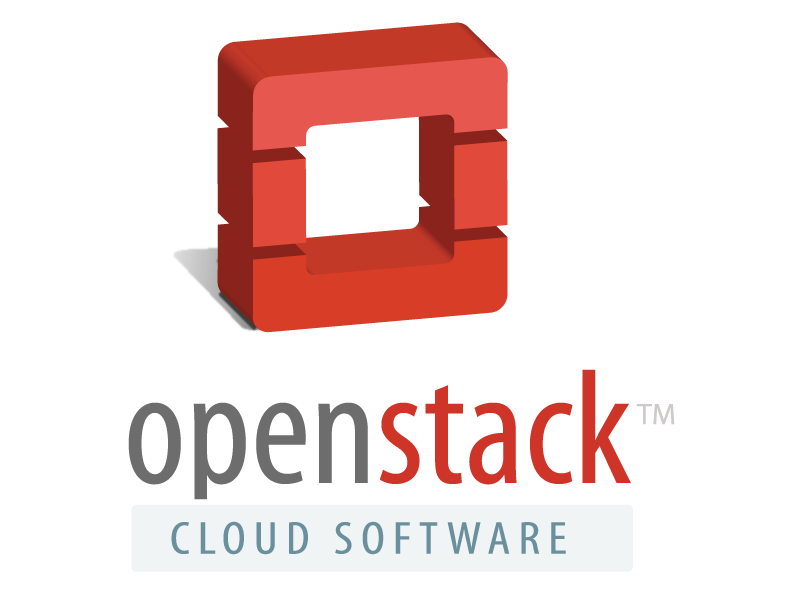
\includegraphics[width=4cm]{openstack.png}
    \end{center}
  \end{frame}

  \AtBeginSection[]
  {
    \begin{frame}[shrink]
      \frametitle{Plan}
      \tableofcontents[currentsection,hideothersubsections]
    \end{frame}
  }
  \AtBeginSubsection[]
  {
    \begin{frame}[shrink]
      \frametitle{Plan}
      \tableofcontents[
        currentsection,
        sectionstyle=show/show,
        subsectionstyle=show/shaded/hide
      ]
    \end{frame}
  }

  \section*{Introduction}
  \begin{frame}
    \frametitle{Objectifs de la formation : Cloud}
    \begin{itemize}
      \item Comprendre les principes du cloud et son intérêt
      \item Connaitre le vocabulaire inhérent au cloud
      \item Avoir une vue d'ensemble sur les solutions existantes en cloud public et privé
      \item Posséder les clés pour tirer partie au mieux de l'IaaS
      \item Pouvoir déterminer ce qui est compatible avec la philosophie cloud ou pas
      \item Adapter ses méthodes d'administration système à un environnement cloud
    \end{itemize}
  \end{frame}

  \begin{frame}
    \frametitle{Objectifs de la formation : OpenStack}
    \begin{itemize}
      \item Connaitre le fonctionnement du projet OpenStack et ses possibilités
      \item Comprendre le fonctionnement de chacun des composants d'OpenStack
      \item Pouvoir faire les bons choix de configuration
      \item Savoir déployer manuellement un cloud OpenStack pour fournir de l'IaaS
      \item Connaitre les bonnes pratiques de déploiement d'OpenStack
      \item Être capable de déterminer l'origine d'une erreur dans OpenStack
      \item Savoir réagir face à un bug
    \end{itemize}
  \end{frame}

  \begin{frame}
    \frametitle{Pré-requis de la formation}
    \begin{itemize}
      \item Compétences d'administration système Linux tel qu'Ubuntu
      \begin{itemize}
        \item Gestion des paquets
        \item LVM et systèmes de fichiers
      \end{itemize}
      \item Notions de virtualisation, KVM et libvirt
      \item Peut servir :
      \begin{itemize}
        \item À l'aise dans un environnement Python
      \end{itemize}
    \end{itemize}
  \end{frame}

  \begin{frame}
    \frametitle{Plan}
    \tableofcontents[hideallsubsections]
  \end{frame}

  \section[Cloud]{Le Cloud : vue d'ensemble}

  \subsection[Cloud]{Le Cloud : les concepts}

  \begin{frame}
    \frametitle{Le cloud, c'est large !}
    \begin{itemize}
      \item Stockage/calcul distant \pause (on oublie, cf. externalisation)\pause
      \item Virtualisation++\pause
      \item Abstraction du matériel (voire plus)\pause
      \item Accès normalisé par des APIs\pause
      \item Service et facturation à la demande\pause
      \item Flexibilité, élasticité
    \end{itemize}
  \end{frame}

  \begin{frame}
    \frametitle{WaaS : Whatever as a Service}
    \begin{itemize}
      \item Principalement\pause
      \begin{description}
        \item[IaaS] \alert<5->{Infrastructure as a Service}\pause
        \item[PaaS] Platform as a Service\pause
        \item[SaaS] Software as a Service\pause
      \end{description}
      \pause
      \item Mais aussi :
      \pause
      \begin{itemize}
        \item Database as a Service
        \item Network as a Service
        \item Load balancing as a Service\pause
        \item \$APPLICATION as a Service
      \end{itemize}
    \end{itemize}
  \end{frame}

  \begin{frame}
    \frametitle{Cloud public ou cloud privé ?}
    \begin{description}
      \item[Public] fourni par un hébergeur à des clients (AWS, Rackspace Cloud, etc.)
      \item[Privé] plateforme et ressources internes
      \item[Hybride] utilisation de ressources publiques au sein d'un cloud privé
    \end{description}
  \end{frame}

  \begin{frame}
    \frametitle{Le cloud en un schéma}
    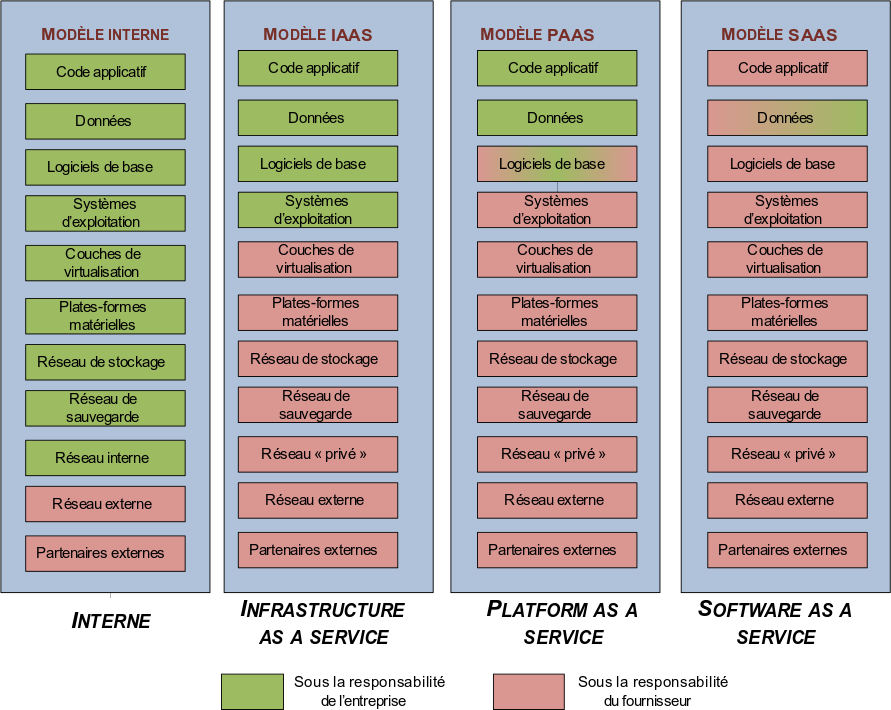
\includegraphics[width=\linewidth,height=\textheight]{cloud.png}
  \end{frame}

  \begin{frame}
    \frametitle{Pourquoi du cloud ? Côté business}
    \begin{itemize}
      \item Baisse des coûts par la mutualisation des ressources
      \item Utilisation uniquement des ressources qui sont nécessaires
      \item À grande échelle, garantie de service
    \end{itemize}
  \end{frame}

  \begin{frame}
    \frametitle{Pourquoi du cloud ? Côté technique}
    \begin{itemize}
      \item Abstraction des couches plus basses
      \item On peut tout programmer à son gré
      \item Permet la mise en place d'architectures scalables
    \end{itemize}
  \end{frame}

  \subsection[PaaS]{PaaS : Platform as a Service}

  \begin{frame}
    \frametitle{PaaS : les principes}
    \begin{itemize}
      \item Fourniture d'une plateforme de développement
      \item Fourniture d'une plateforme de déploiement
      \item Pour un langage / un framework
      \item Principalement utilisé par des développeurs
    \end{itemize}
  \end{frame}

  \begin{frame}
    \frametitle{Exemples de PaaS publics}
    \begin{itemize}
      \item Amazon OpsWork / Elastic Beanstalk
      \item Google App Engine
      \item Heroku
    \end{itemize}
  \end{frame}

  \begin{frame}
    \frametitle{Solutions de PaaS privé}
    \begin{itemize}
      \item Cloud Foundry
      \item OpenShift (Red Hat)\pause
      \item Solum
    \end{itemize}
  \end{frame}

  \subsection[IaaS]{IaaS : Infrastructure as a Service}

  \begin{frame}
    \frametitle{Amazon Web Services (AWS) et les autres}
    \begin{itemize}
      \item Service (cloud public) : \textcolor{blue}{AWS}
      \begin{itemize}
        \item Pionnier du genre (dès 2002)\pause
        \item Elastic Compute Cloud (\textcolor{blue}{EC2})
        \item Elastic Block Storage (\textcolor{blue}{EBS})\pause
        \item Simple Storage Service (\textcolor{blue}{S3})\pause
      \end{itemize}
        \item Logiciels libres permettant le déploiement d'un cloud privé :
      \begin{itemize}
        \item Eucalyptus
        \item CloudStack
        \item OpenNebula\pause
        \item \textbf{OpenStack}
      \end{itemize}
    \end{itemize}
  \end{frame}

  \begin{frame}
    \frametitle{Les clouds publics concurrents d'AWS}
    \begin{itemize}
      \item Google Compute Platform
      \item \textbf<3->{Rackspace}
      \item \textbf<3->{HP Cloud}\pause
      \item En France
      \begin{itemize}
        \item \textbf<3->{Cloudwatt}
        \item \textbf<3->{Numergy}
      \end{itemize}
    \end{itemize}
  \end{frame}

  \begin{frame}
    \frametitle{Virtualisation dans le cloud}
    \begin{itemize}
      \item Le cloud IaaS repose souvent sur la virtualisation
      \item Ressources compute $\leftarrow$ virtualisation
      \item Virtualisation complète : KVM, Xen
      \item Virtualisation containers : OpenVZ, LXC, Docker
    \end{itemize}
  \end{frame}

  \begin{frame}
    \frametitle{Notions et vocabulaire IaaS}
    \begin{itemize}
      \item Images
      \item Instances
      \item Types d'instance (flavors)
      \item Volumes\pause
      \item Stockage block
      \item Stockage objet\pause
      \item IP flottantes/élastiques\pause
      \item Groupes de sécurité\pause
      \item Paires de clés\pause
      \item API REST\pause
      \item API de metadata et user data
      \item Cloud-init
    \end{itemize}
  \end{frame}

  \begin{frame}
    \frametitle{Notions et vocabulaire IaaS}
    \begin{itemize}
      \item L'instance est par définition éphémère
      \item Elle doit être utilisée comme ressource de calcul
      \item Une image se personnalise lors de son instanciation grâce à l'API de metadata
      \item Séparer les données des instances
      \item Choix du type de stockage : éphémère, volume, objet
    \end{itemize}
  \end{frame}

  \begin{frame}
    \frametitle{À retenir}
    \Huge{Virtualisation $\ne$ IaaS}
  \end{frame}

  \begin{frame}
    \frametitle{AWS}
    \huge{Regardons l'interface web d'Amazon}
  \end{frame}

  \subsection[Stockage]{Stockage : block, objet, SDS}

  \begin{frame}
    \frametitle{Stockage block}
    \begin{itemize}
      \item Accès à des raw devices type \textit{/dev/vdb}
      \item Possibilité d'utiliser n'importe quel système de fichiers
      \item Compatible avec toutes les applications legacy
    \end{itemize}
  \end{frame}

  \begin{frame}
    \frametitle{Stockage objet}
    \begin{itemize}
      \item Pousser et retirer des objets dans un container/bucket
      \item Pas de hiérarchie des données, pas de système de fichiers
      \item Accès par les APIs
      \item L'application doit être conçue pour tirer partie du stockage objet
    \end{itemize}
  \end{frame}

  \begin{frame}
    \frametitle{Stockage objet : schéma}
    \begin{center}
      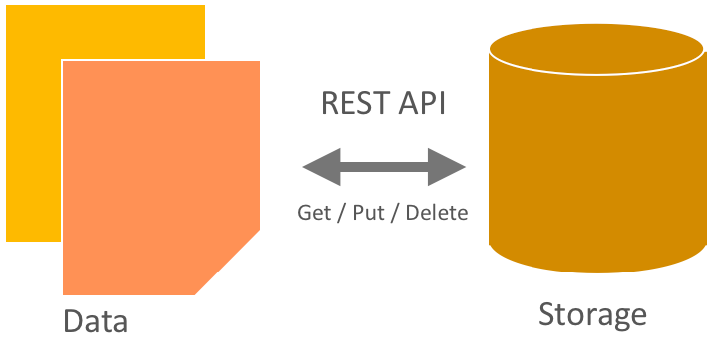
\includegraphics{stockage-objet.png}
    \end{center}
  \end{frame}

  \begin{frame}
    \frametitle{SDS : Software Defined Storage}
    \begin{itemize}
      \item Utilisation de commodity hardware
      \item Pas de RAID matériel
      \item Le logiciel est responsable de garantir les données
    \end{itemize}
  \end{frame}

  \begin{frame}
    \frametitle{Deux solutions : OpenStack Swift et Ceph}
    \begin{itemize}
      \item Swift fait partie du projet OpenStack et fournit du stockage objet
      \item Ceph fournit du stockage objet, block et FS
      \item Les deux sont du SDS
      \item Théorème CAP : on en choisit deux
    \end{itemize}
  \end{frame}

  \begin{frame}
  \frametitle{Théorème CAP}
  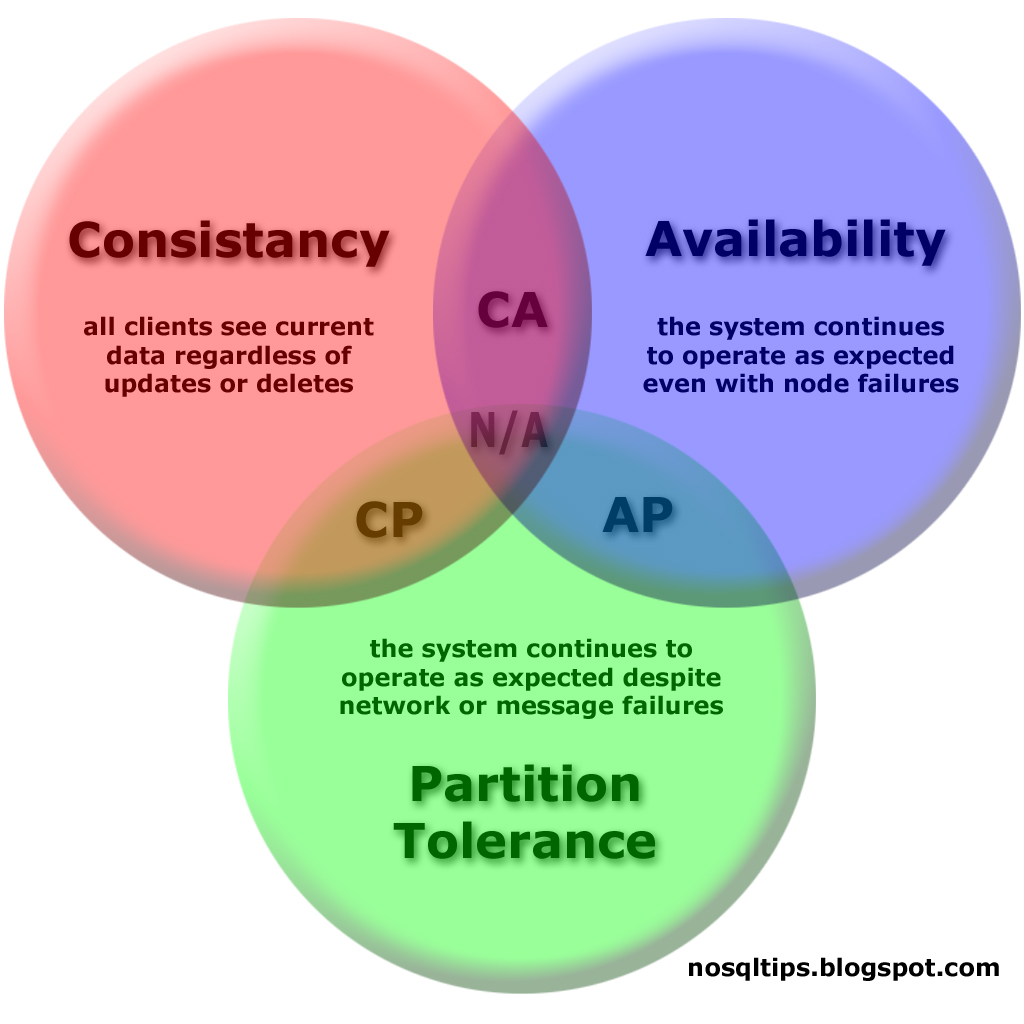
\includegraphics[width=\textwidth,height=\textheight]{cap.jpg}
  \end{frame}

  \begin{frame}
  \frametitle{Swift}
    \begin{itemize}
      \item Swift est un projet OpenStack
      \item Le projet est né chez Rackspace avant la création d'OpenStack
      \item Swift est en production chez Rackspace depuis lors
      \item C'est le composant le plus mature d'OpenStack
    \end{itemize}
  \end{frame}

  \begin{frame}
  \frametitle{Ceph}
    \begin{itemize}
      \item Projet totalement parallèle à OpenStack
      \item Supporté par une entreprise (Inktank) récemment rachetée par Red Hat
      \item Fournit d'abord du stockage objet
      \item L'accès aux données se fait via RADOS :
      \begin{itemize}
        \item Accès direct depuis une application avec librados
        \item Accès via une API REST grâce à radosgw
      \end{itemize}
      \item La couche RBD permet d'accéder aux données en mode block (volumes)
      \item CephFS permet un accès par un système de fichiers POSIX
    \end{itemize}
  \end{frame}

  \subsection[Orchestration]{Orchestrer les ressources de son IaaS}

  \begin{frame}
    \frametitle{Pourquoi orchestrer}
    \begin{itemize}
      \item Définir tout une infrastructure dans un seul fichier texte
      \item Être en capacité d'instancier une infrastructure entière en un appel API
      \item Adapter ses ressources en fonction de ses besoins en temps réel (autoscaling)
    \end{itemize}
  \end{frame}

  \subsection[APIs]{APIs : quel rôle ?}

  \begin{frame}
    \frametitle{API ?}
    \begin{itemize}
      \item \textit{Application Programming Interface}
      \item Au sens logiciel : Interface permettant à un logiciel d'utiliser une bibliothèque
      \item Au sens cloud : Interface permettant à un logiciel d'utiliser un service (XaaS)
      \item Il s'agit le plus souvent d'API HTTP REST
    \end{itemize}
  \end{frame}

  \begin{frame}[containsverbatim]
    \frametitle{Exemple concret}
\begin{verbatim}
GET /v2.0/networks/network_id
{
   "network":{
      "status":"ACTIVE",
      "subnets":[
         "54d6f61d-db07-451c-9ab3-b9609b6b6f0b"
      ],
      "name":"private-network",
      "provider:physical_network":null,
      "admin_state_up":true,
      "tenant_id":"4fd44f30292945e481c7b8a0c8908869",
      "provider:network_type":"local",
      "router:external":true,
      "shared":true,
      "id":"d32019d3-bc6e-4319-9c1d-6722fc136a22",
      "provider:segmentation_id":null
   }
}
\end{verbatim}
  \end{frame}

  \section[OpenStack]{OpenStack : projet, logiciel et utilisation}

  \subsection[OpenStack]{Présentation du projet et du logiciel}

  \begin{frame}
    \frametitle{Vue haut niveau}
    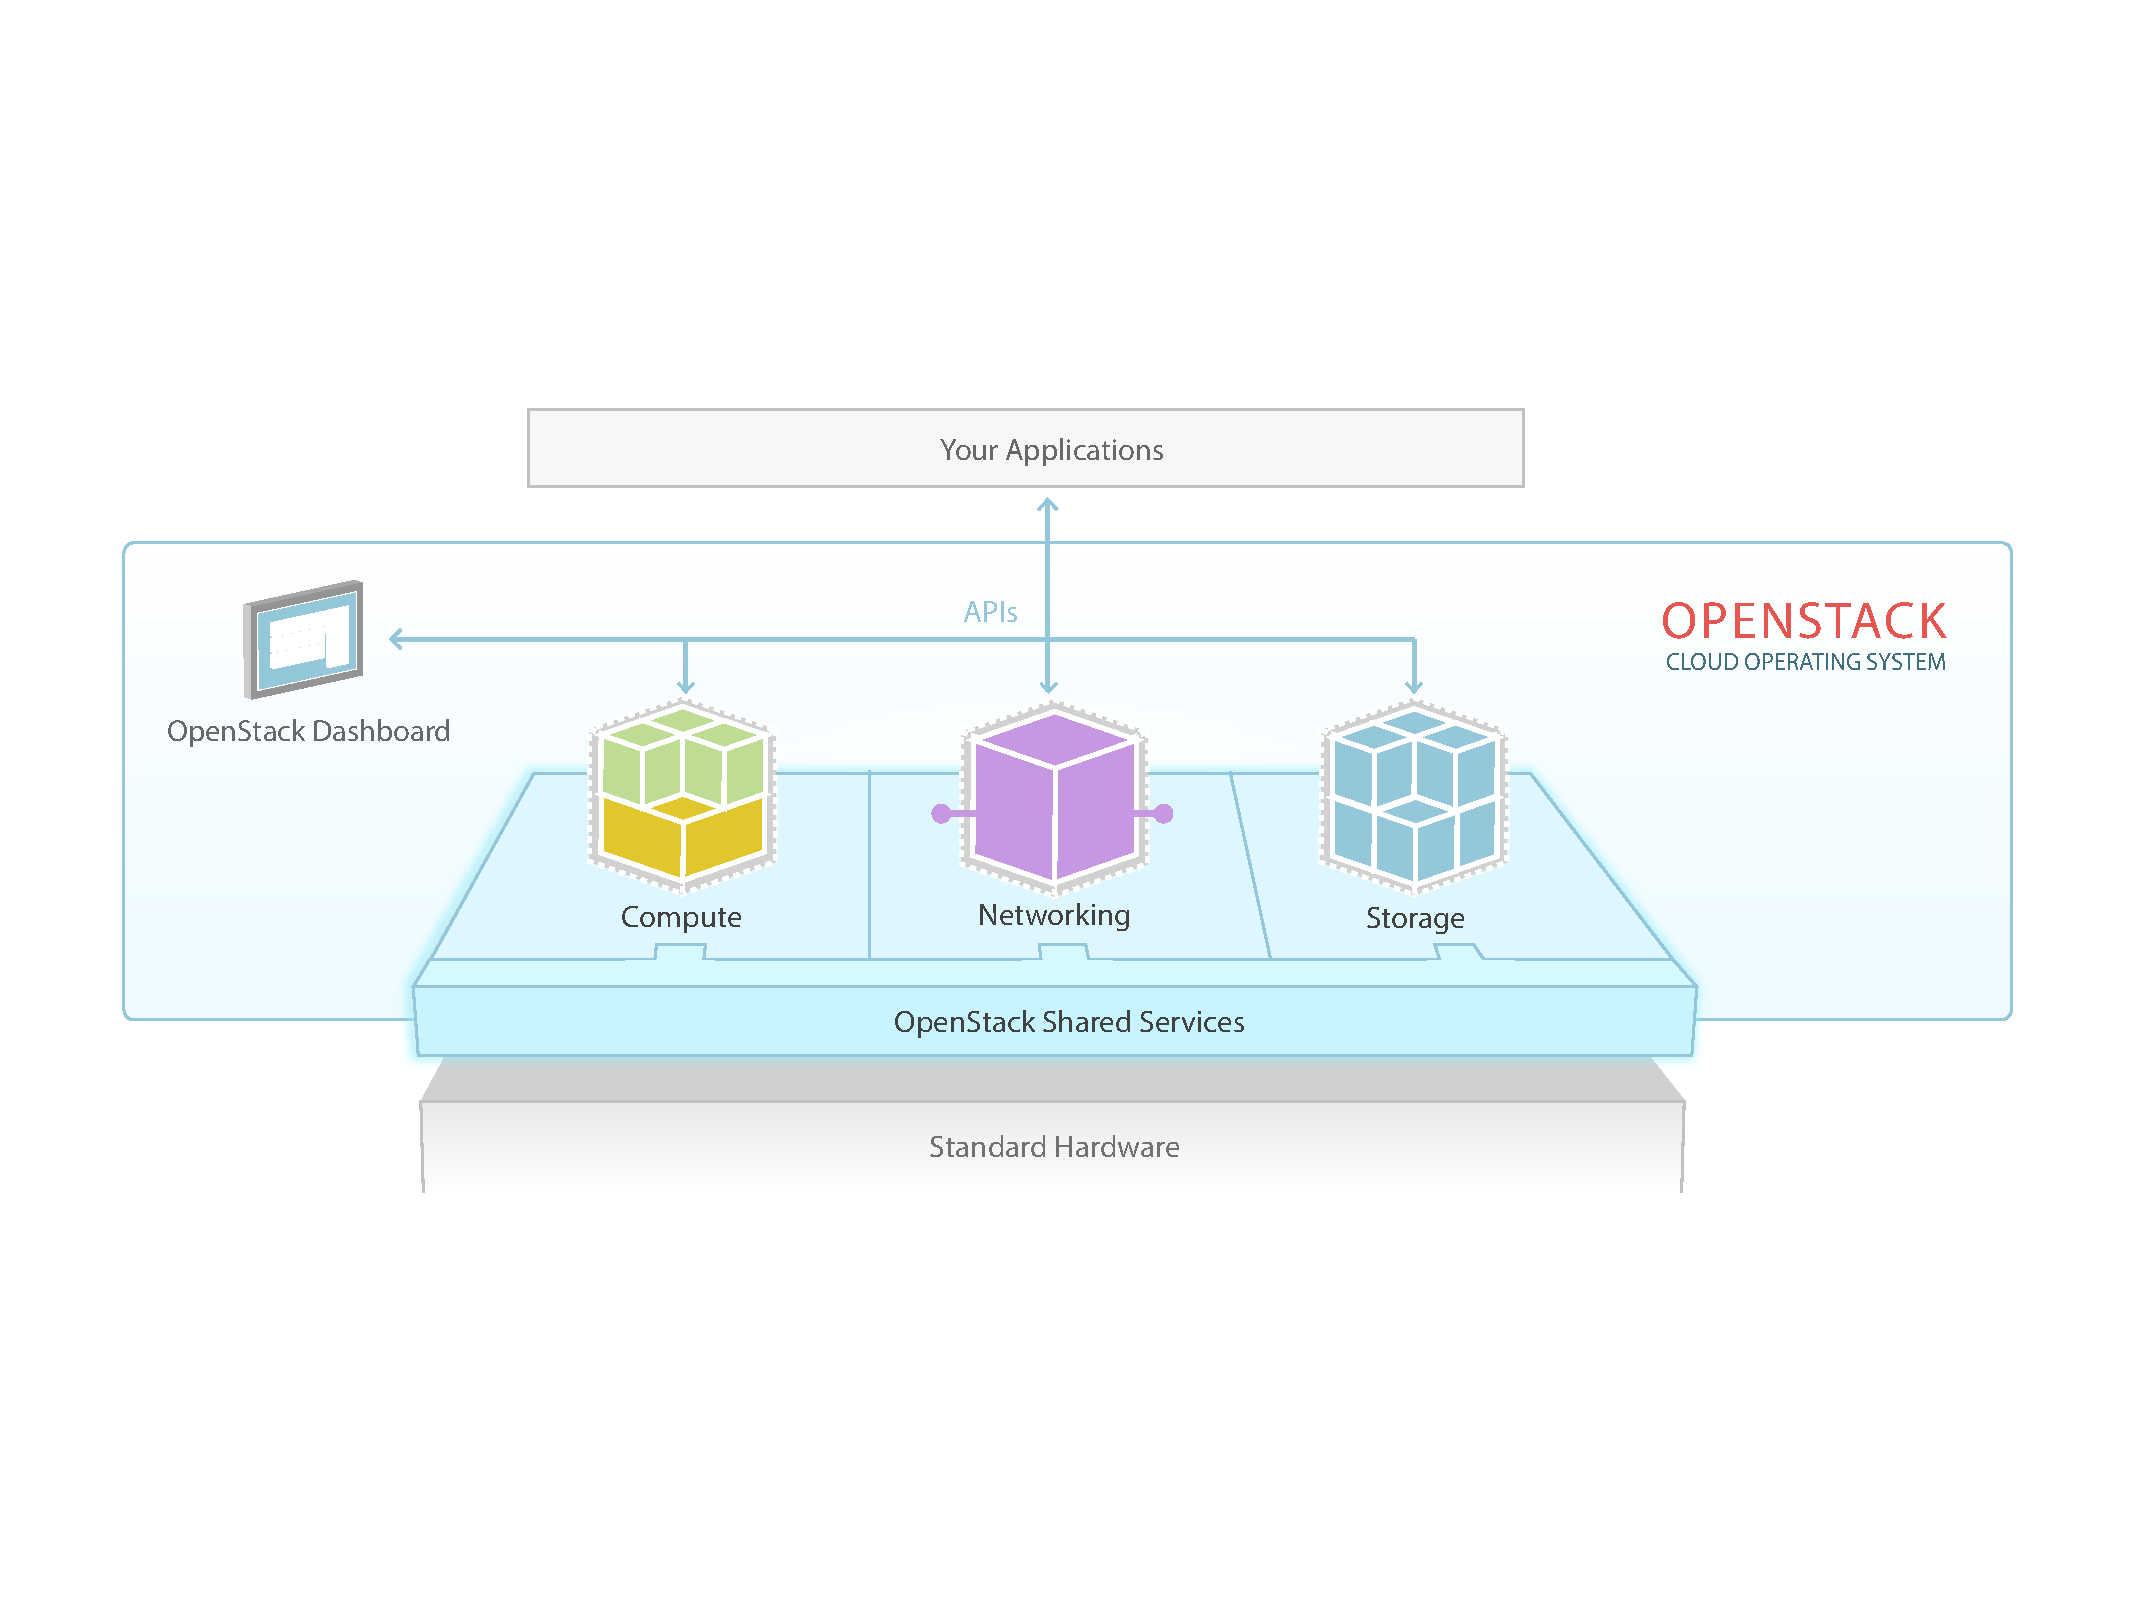
\includegraphics[width=\textwidth]{openstack-software-diagram.pdf}
  \end{frame}

  \begin{frame}
    \frametitle{Historique}
    \begin{itemize}
      \item Démarrage en 2010
      \item Objectif : le Cloud Operating System libre
      \item Fusion de deux projets de Rackspace (Storage) et de la NASA (Compute)
      \item Développé en Python et distribué sous licence Apache 2.0\pause
      \item Les releases jusqu'à aujourd'hui :
      \begin{itemize}
        \item Austin (2010.1)
        \item Bexar (2011.1)
        \item Cactus (2011.2)
        \item Diablo (2011.3)
        \item Essex (2012.1)
        \item Folsom (2012.2)
        \item Grizzly (2013.1)
        \item Havana (2013.2)
        \item \textbf{Icehouse (2014.1)}\pause
        \item Novembre 2014 : Juno
      \end{itemize}
    \end{itemize}
  \end{frame}

  \begin{frame}
    \frametitle{Quelques soutiens/contributeurs ...}
    \begin{itemize}
      \item \textcolor{blue}{Rackspace} et la NASA\pause
      \item \textcolor{blue}{Canonical}
      \item \textcolor{blue}{Red Hat}
      \item \textcolor{blue}{Suse}\pause
      \item \textcolor{blue}{HP}
      \item \textcolor{blue}{IBM}
      \item \textcolor{cyan}{Dell}, \textcolor{cyan}{Intel}
      \item \textcolor{cyan}{Cisco}, \textcolor{cyan}{Juniper}\pause
      \item \textcolor{cyan}{NetApp}, \textcolor{cyan}{VMWare}\pause
      \item \textcolor{cyan}{Yahoo}, Bull\pause
      \item Mais aussi : Mirantis, StackOps, \textcolor{cyan}{eNovance}\pause
    \end{itemize}
    \url{http://www.openstack.org/foundation/companies/}
  \end{frame}

  \begin{frame}
    \frametitle{... et utilisateurs}
    \begin{itemize}
      \item Tous les contributeurs précédemment cités\pause
      \item En France : \textbf{CloudWatt} et \textbf{Numergy}\pause
      \item Wikimedia
      \item CERN
      \item Paypal
      \item Comcast\pause
      \item Etc. Sans compter les implémentations confidentielles
    \end{itemize}
    \url{http://www.openstack.org/user-stories/}
  \end{frame}

  \begin{frame}
    \frametitle{Les différents sous-projets}
    \begin{itemize}
        \item OpenStack Compute - Nova
        \item OpenStack (Object) Storage - Swift\pause
        \item OpenStack Block Storage - Cinder\pause
        \item OpenStack Networking - Neutron\pause
        \item OpenStack Image Service - Glance\pause
        \item OpenStack Identity Service - Keystone\pause
        \item OpenStack Dashboard - Horizon\pause
        \item OpenStack Metering - Ceilometer\pause
        \item OpenStack Orchestration - Heat\pause
        \item OpenStack Database Service - Trove
    \end{itemize}
  \end{frame}

  \begin{frame}
    \frametitle{Les différents sous-projets (2)}
    \begin{itemize}
      \item Incubating (à jour Icehouse)
      \begin{itemize}
        \item Bare metal (Ironic)
        \item Queue service (Marconi)
        \item Data processing (Sahara)
      \end{itemize}\pause
      \item Intéressants
      \begin{itemize}
        \item DNS service (Designate)
      \end{itemize}
      \item Autres\pause
      \begin{itemize}
        \item Oslo
        \item rootwrap : wrapper pour les commandes root utilisé par les projets
        \item TripleO
        \item Tempest, Grenade
        \item Les clients (python-*client)
      \end{itemize}
    \end{itemize}
  \end{frame}

  \begin{frame}
    \frametitle{Cycle de vie des projets au sein d'OpenStack}
    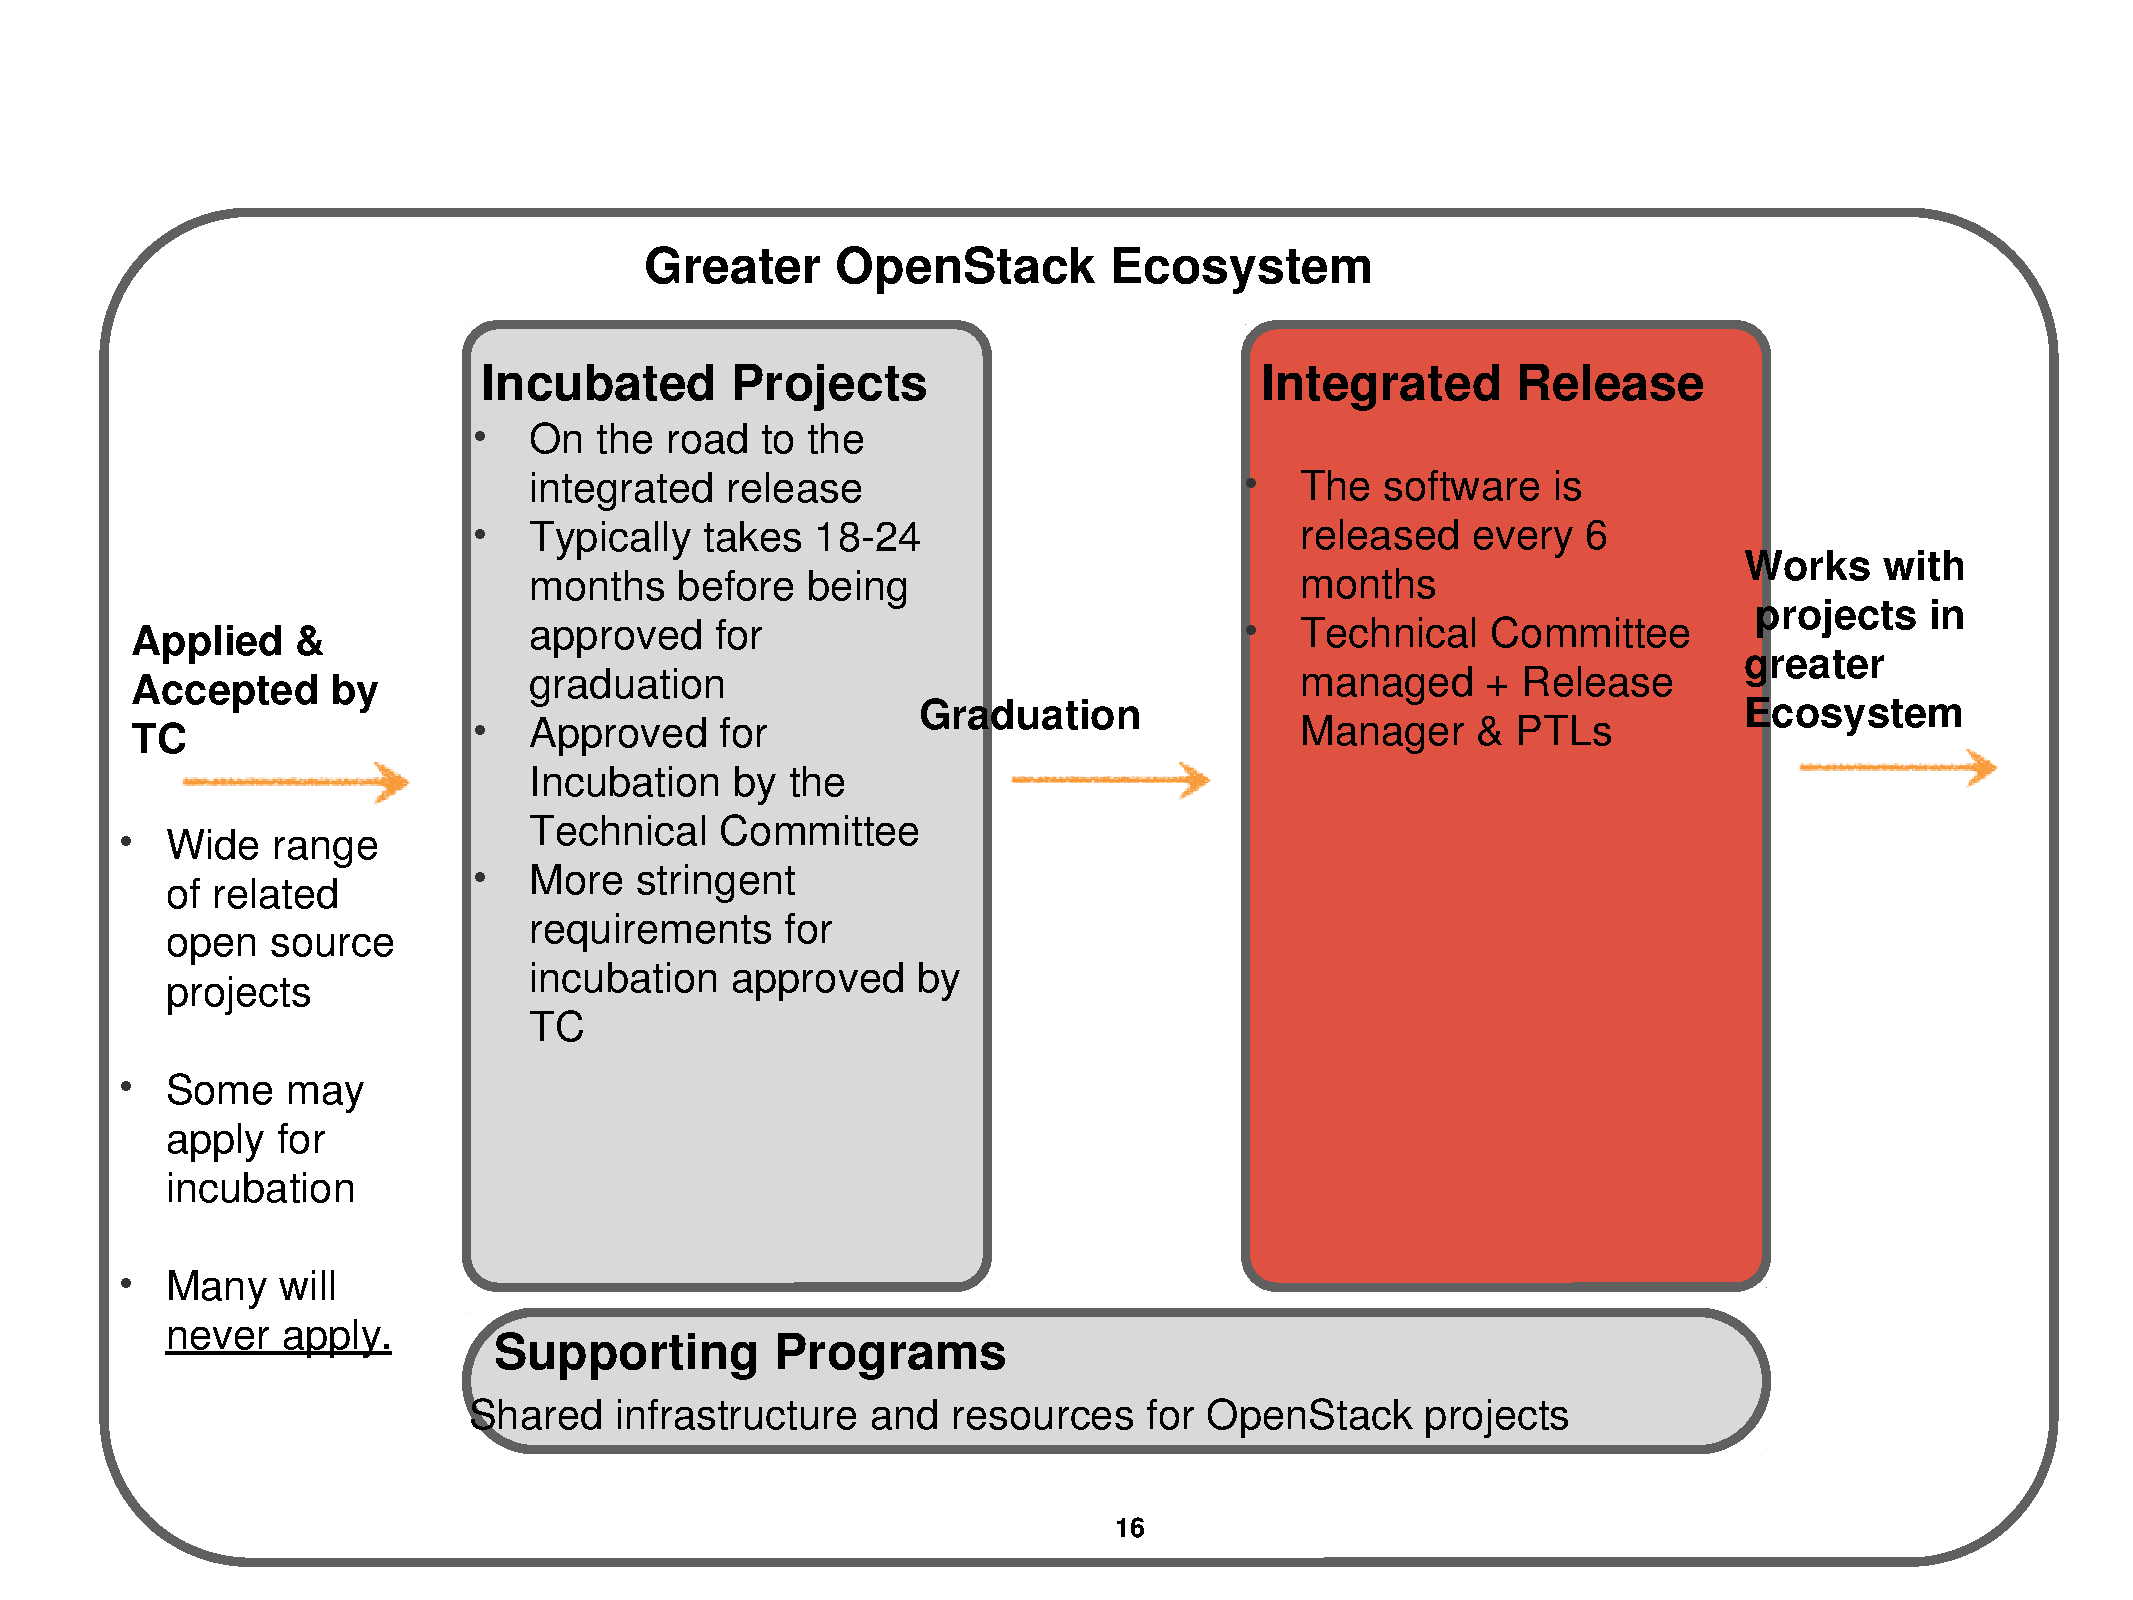
\includegraphics[width=\textwidth]{innovation1.pdf}
  \end{frame}

  \begin{frame}
    \frametitle{Les projets dans Icehouse}
    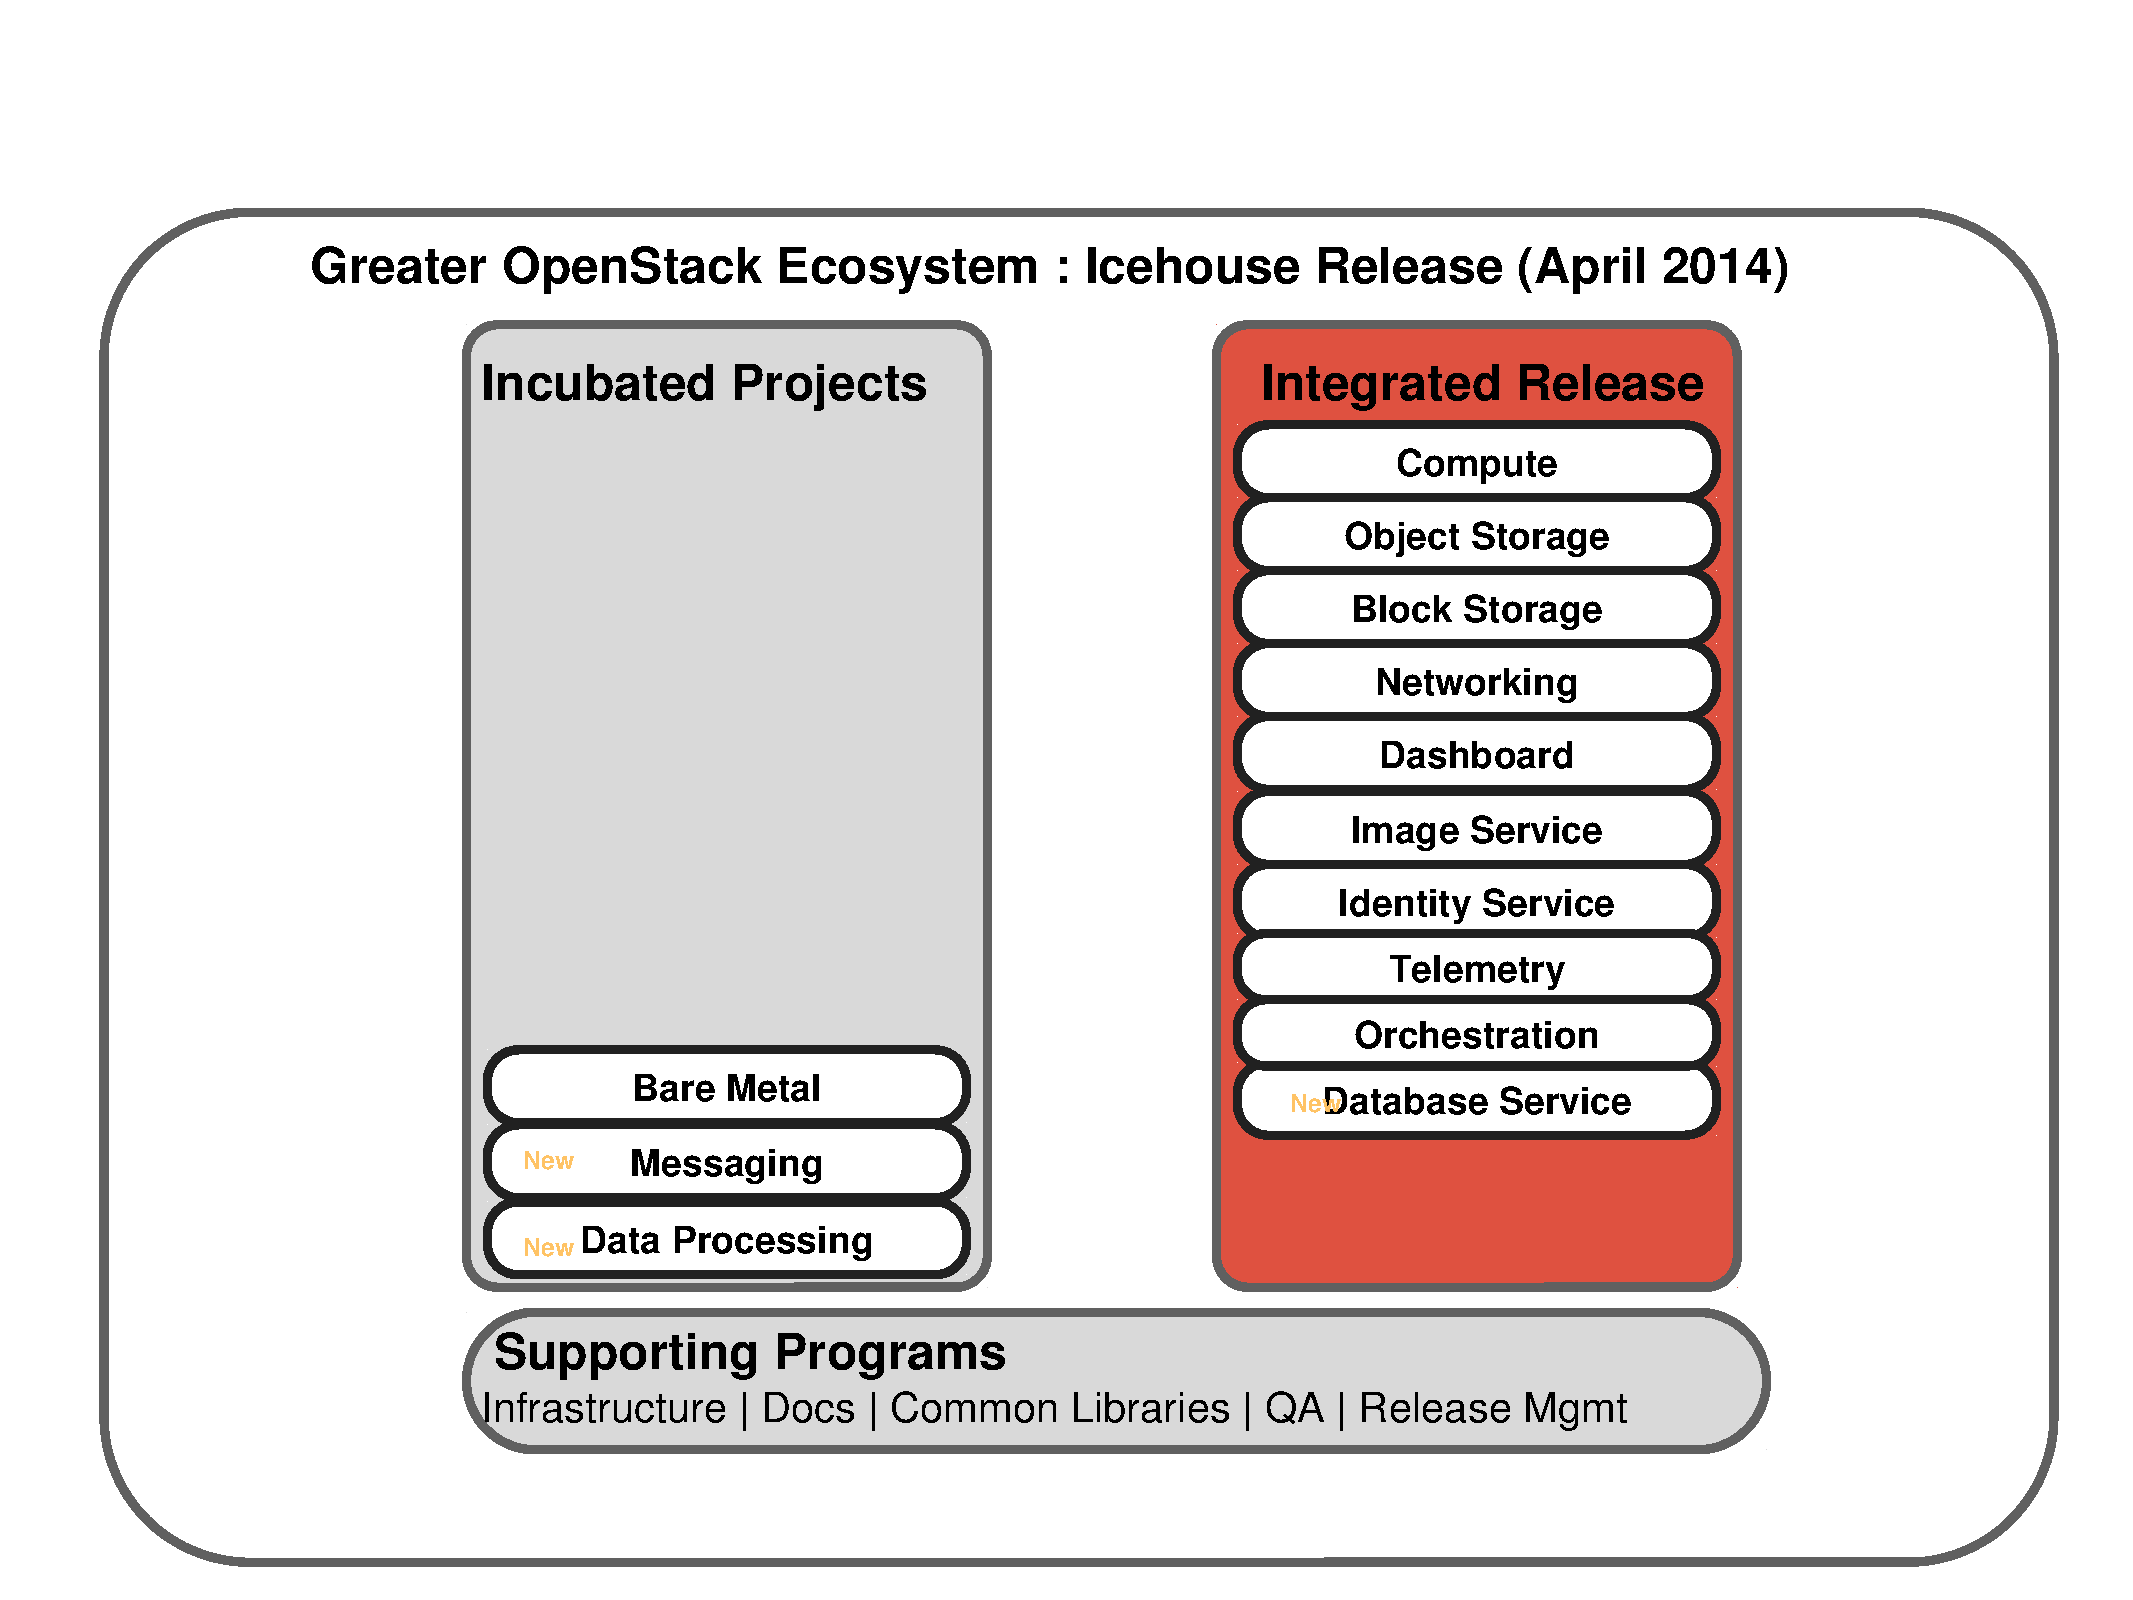
\includegraphics[width=\textwidth]{innovation2.pdf}
  \end{frame}

  \begin{frame}
    \frametitle{Nouveautés de Icehouse}
    \begin{center}
      
\includegraphics{icehouse.png}
    \end{center}
    \begin{itemize}
      \item Nova : rolling upgrades
      \item Nouvelles fonctionnalités disponibles dans Horizon
      \item Nouveaux drivers dans Neutron
      \item Nouveaux drivers dans Cinder
      \item Le nouveau format HOT est recommandé pour les templates Heat
      \item etc.
      \item En détails : \url{https://wiki.openstack.org/wiki/ReleaseNotes/Icehouse}
    \end{itemize}
  \end{frame}

  \begin{frame}
    \frametitle{Traduction}
    \begin{itemize}
      \item La question de la traduction est dorénavant prise en compte
      \item Seules certaines parties sont traduites, comme Horizon
      \item La traduction française est aujourd'hui une des plus avancées
      \item Utilisation de la plateforme Transifex
    \end{itemize}
  \end{frame}

  \begin{frame}
    \frametitle{Développement du projet}
    \begin{itemize}
      \item Open Source
      \item Open Design
      \item Open Development
      \item Open Community
    \end{itemize}
  \end{frame}

  \begin{frame}
    \frametitle{Développement du projet : en détails}
    \begin{itemize}
      \item Ouvert à tous (individuels et entreprises)\pause
      \item Cycle de développement de 6 mois débuté par un (design) summit\pause
      \item Outils : Launchpad (blueprints, bugs) + Git + GitHub (code)\pause
      \item Sur chaque commit : peer review (Gerrit) + intégration continue (exécution de différents tests par Jenkins)\pause
      \item Plateforme de référence et modèle de développement : Ubuntu\pause
      \item Développement hyper actif : 17000 commits dans Icehouse (+25\%)\pause
      \item Fin 2012, création d'une entité indépendante de gouvernance : la fondation OpenStack
    \end{itemize}
  \end{frame}

  \begin{frame}
    \frametitle{La fondation OpenStack}
    \begin{itemize}
      \item Entité de gouvernance principale du projet
      \item Les membres du board sont issus des entreprises sponsors et élus par les membres individuels
      \item Tout le monde peut devenir membre individuel (gratuitement)
      \item La fondation supporte le projet par différents moyens :
      \begin{itemize}
        \item Événements : organisation (Summits) ou participation (OSCON, etc.)
        \item Infrastructure de développement (serveurs)
        \item Ressources humaines : marketing, release manager, quelques développeurs (principalement sur l'infrastructure)
      \end{itemize}
      \item 850 organisations à travers le monde
      \item 9500 membres individuels dans 100 pays
    \end{itemize}
  \end{frame}

  \begin{frame}
    \frametitle{La fondation OpenStack}
      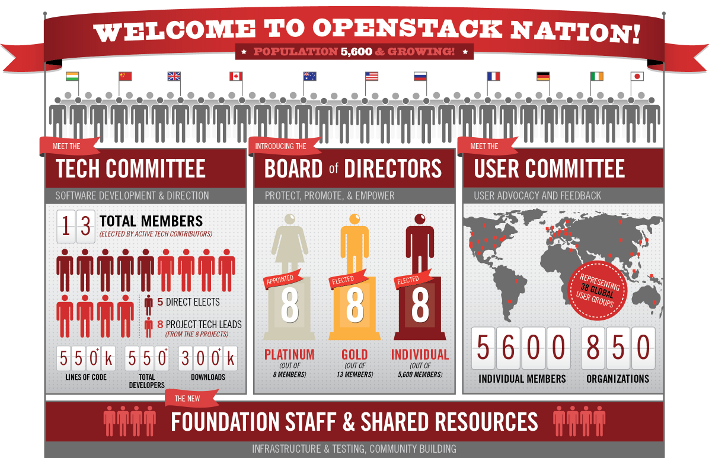
\includegraphics[width=\textwidth]{foundation.png}
  \end{frame}

  \begin{frame}
    \frametitle{Cycle de développement : 6 mois}
    \begin{itemize}
      \item Le planning est publié, exemple : \url{https://wiki.openstack.org/wiki/Icehouse_Release_Schedule}
      \item Milestone releases
      \item Freezes : FeatureProposal, Feature, String
      \item RC releases
      \item Stable releases
      \item Ce modèle de cycle de développement a évolué depuis le début du projet
      \item Cas particulier de Swift
    \end{itemize}
  \end{frame}

  \begin{frame}
    \frametitle{Où trouver des informations sur le développement d'OpenStack}
    \begin{itemize}
      \item Principalement sur le wiki : \url{https://wiki.openstack.org}
      \item Les blueprints et bugs sur Launchpad : \url{https://launchpad.net/openstack}
      \item Les patchs proposés et leurs reviews sont sur Gerrit : \url{https://review.openstack.org}
      \item Le code est disponible dans Git : \url{https://git.openstack.org}
      \item Les sources (tarballs) sont disponibles : \url{http://tarballs.openstack.org/}
    \end{itemize}
  \end{frame}

  \begin{frame}
    \frametitle{Stackforge}
    \begin{itemize}
      \item Forge pour les nouveaux projets en lien avec OpenStack
      \item Ils bénéficient de l'infrastructure du projet OpenStack, mais la séparation reste claire
      \item Les projets démarrent dans Stackforge et peuvent ensuite rejoindre le projet OpenStack
    \end{itemize}
  \end{frame}

  \begin{frame}
    \frametitle{OpenStack Summit}
    \begin{itemize}
      \item Aux USA jusqu'en 2013
      \item Aujourd'hui : alternance USA et Asie/Europe
      \item Quelques centaines au début à 4500 de participants aujourd'hui
      \item En parallèle : conférence (utilisateurs, décideurs) et Design Summit (développeurs)
      \item Détermine le nom de la release : lieu/ville à proximité du Summit
    \end{itemize}
  \end{frame}

  \begin{frame}
    \frametitle{Exemple du Summit d'avril 2013 à Portland}
    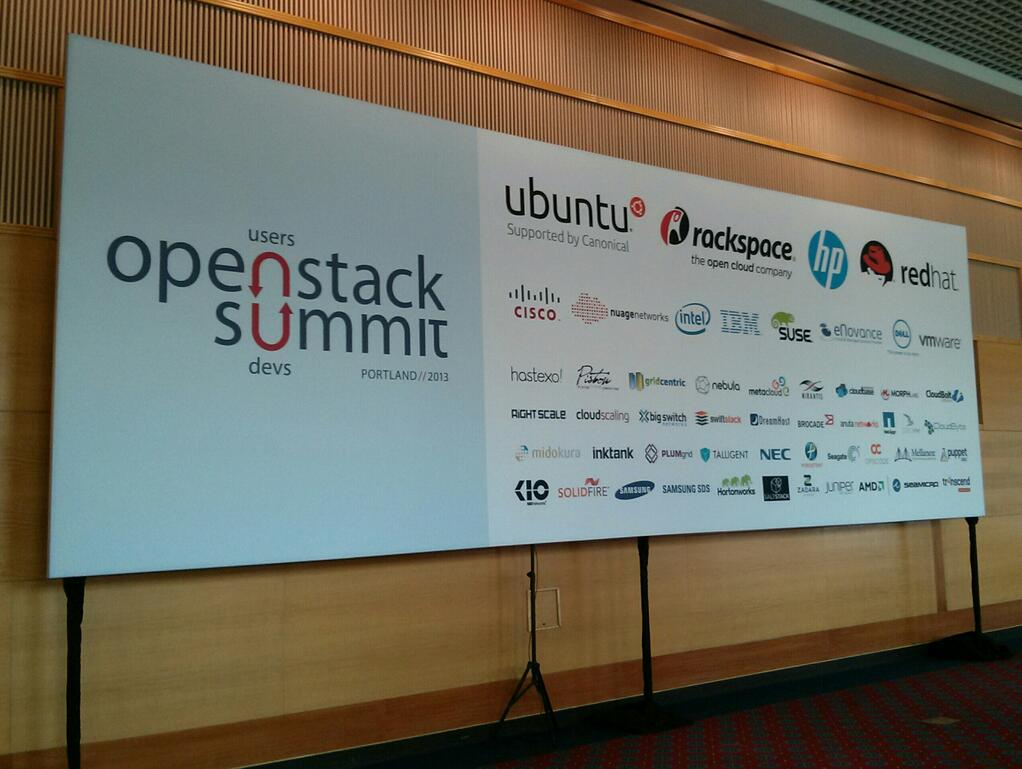
\includegraphics[width=\textwidth]{photo-summit.jpg}
  \end{frame}

  \begin{frame}
    \frametitle{Exemple du Summit de mai 2014 à Atlanta}
    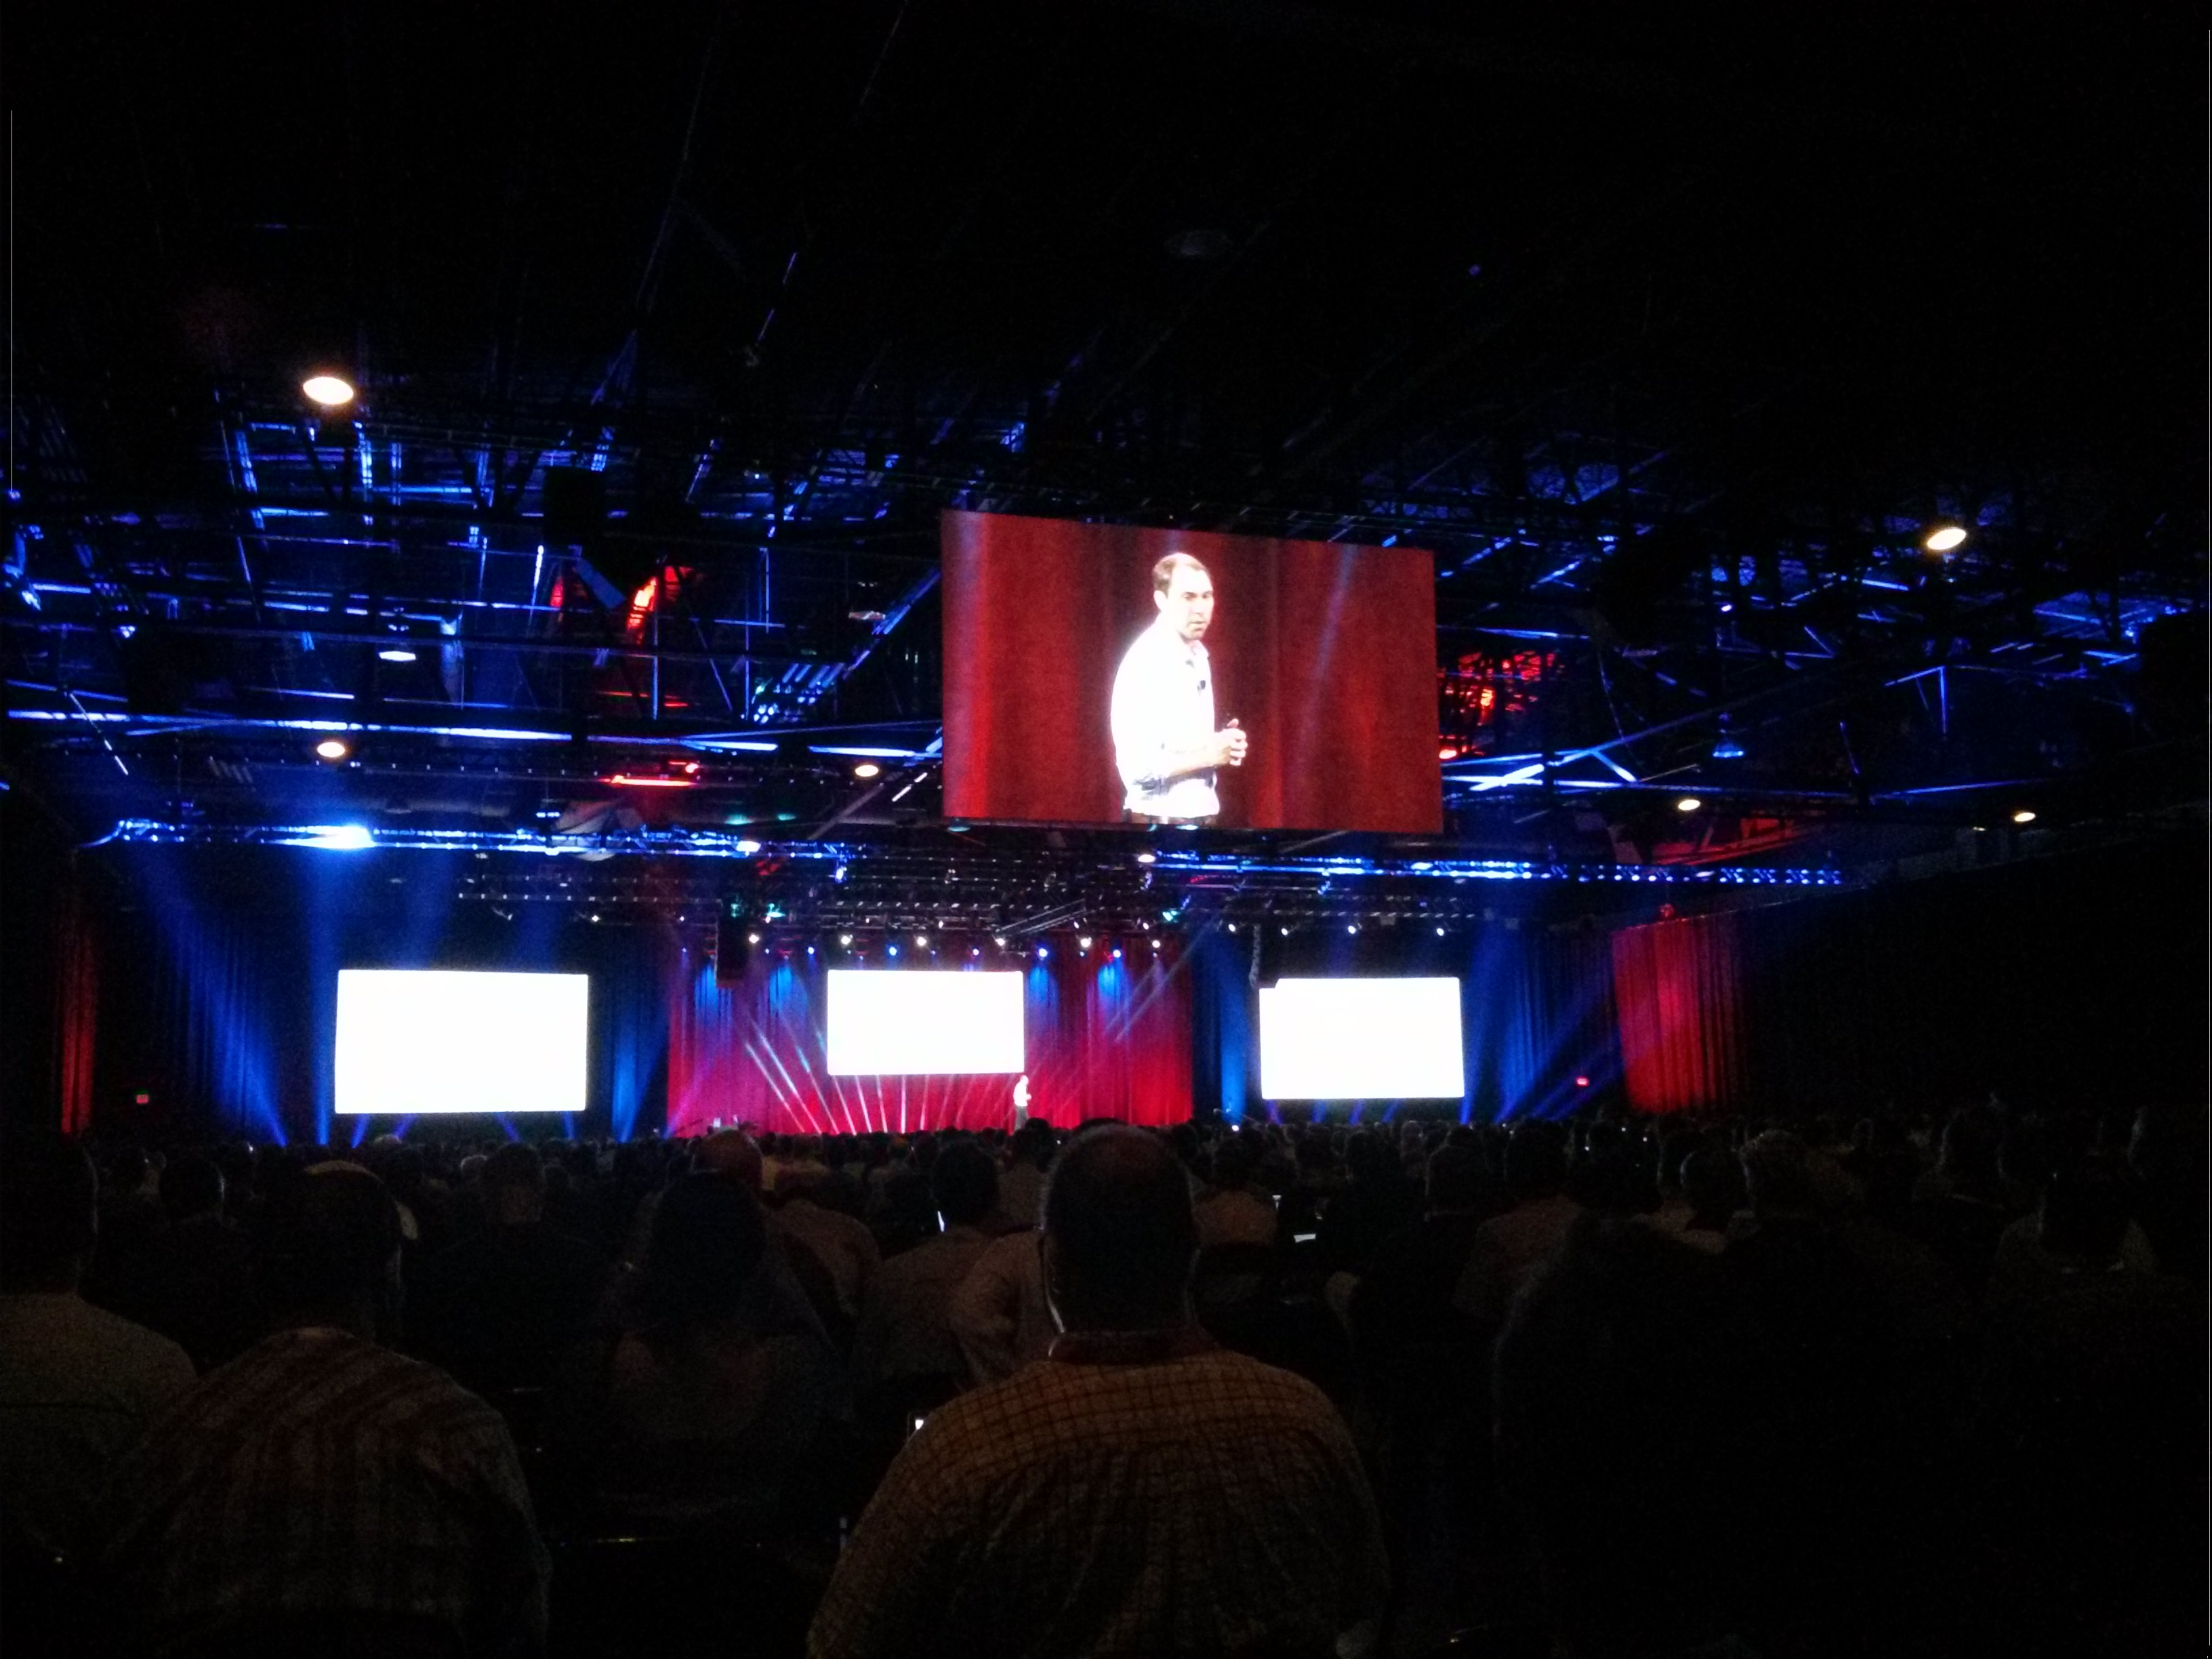
\includegraphics[width=\textwidth]{photo-summit1.jpg}
  \end{frame}

  \begin{frame}
    \frametitle{Exemple du Summit de mai 2014 à Atlanta}
    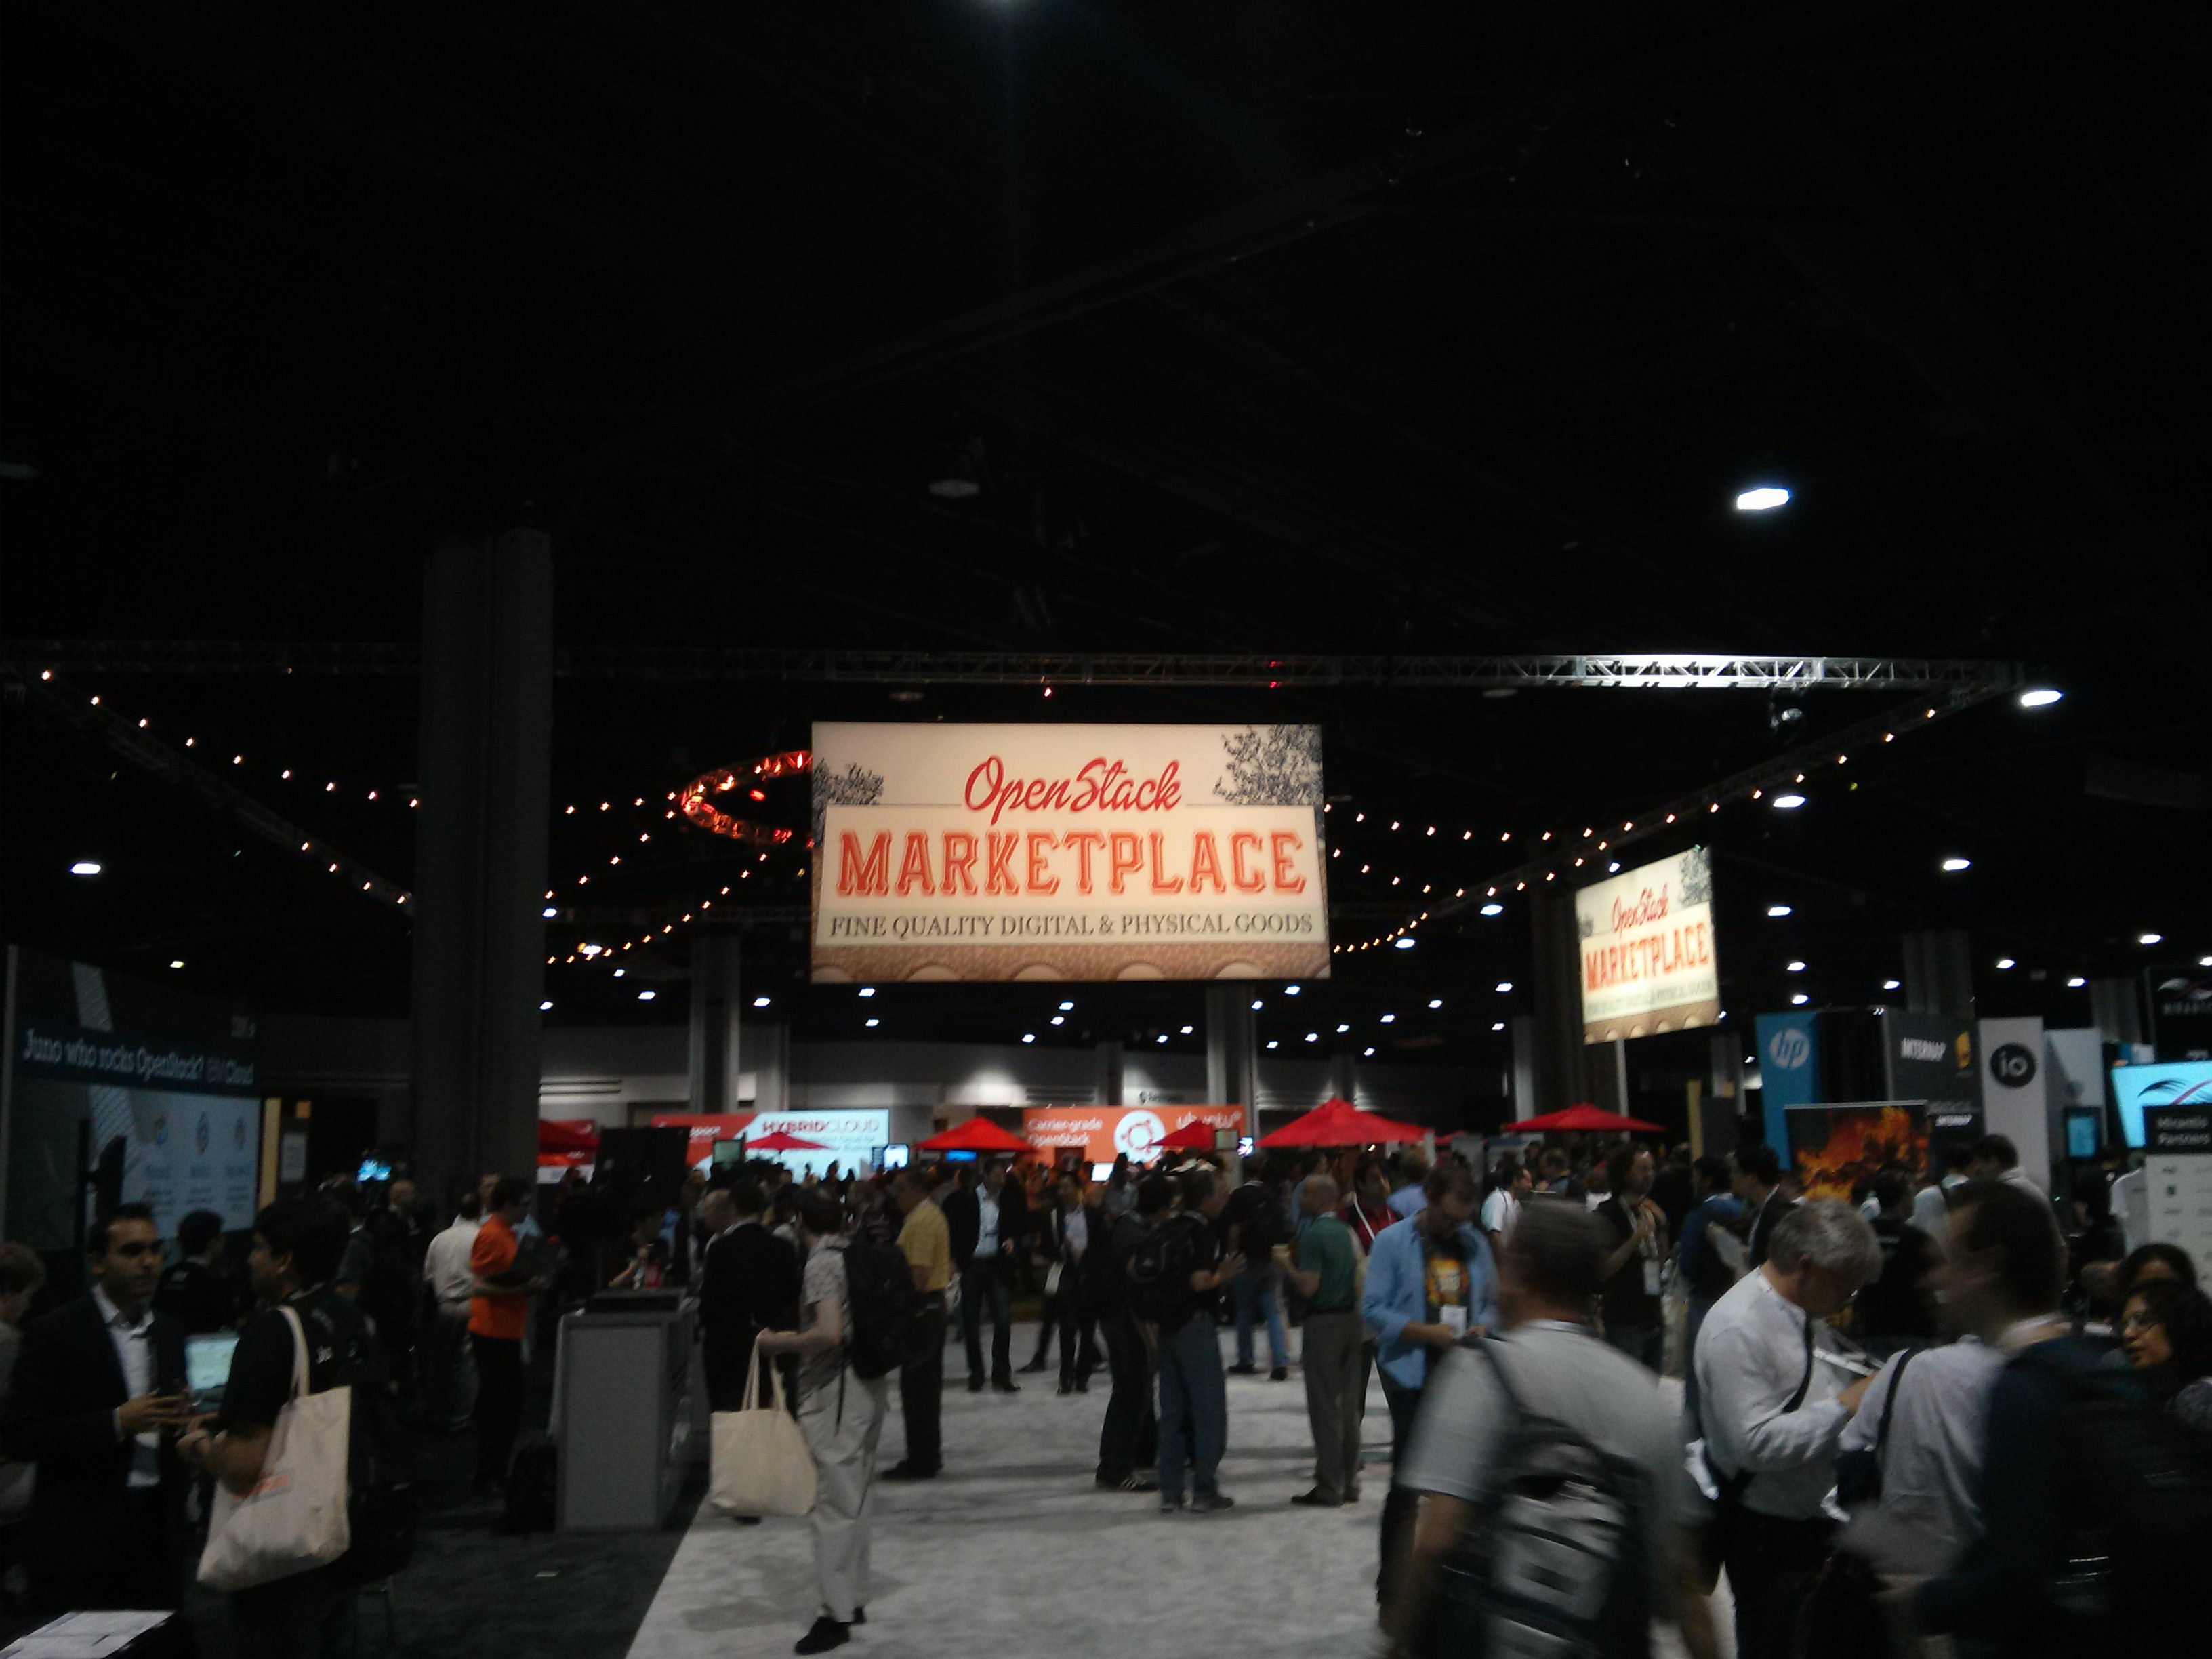
\includegraphics[width=\textwidth]{photo-summit2.jpg}
  \end{frame}
  \begin{frame}
    \frametitle{Design Tenets}
    \begin{enumerate}
      \item Scalability and elasticity are our main goals
      \item Any feature that limits our main goals must be optional
      \item Everything should be asynchronous. If you can't do something asynchronously, see \#2
      \item All required components must be horizontally scalable
      \item Always use shared nothing architecture (SN) or sharding. If you can't Share nothing/shard, see \#2
      \item Distribute everything. Especially logic. Move logic to where state naturally exists.
      \item Accept eventual consistency and use it where it is appropriate.
      \item Test everything. We require tests with submitted code. (We will help you if you need it)
    \end{enumerate}
  \end{frame}

  \begin{frame}
    \frametitle{Implémentation}
    \begin{itemize}
      \item Chaque sous-projet est découpé en plusieurs services\pause
      \item Communication entre les services : AMQP (RabbitMQ)\pause
      \item Base de données : MySQL\pause
      \item Réutilisation de nombreux composants existants\pause
      \item OpenVSwitch\pause
      \item Tout est développé en Python (Django pour Horizon)\pause
      \item APIs supportées : OpenStack et équivalent Amazon\pause
      \item Multi tenancy
    \end{itemize}
  \end{frame}

  \begin{frame}
    \frametitle{Multi-tenant}
    \begin{itemize}
      \item Notion générale : un déploiement du logiciel permet de multiples utilisations
      \item Un cloud OpenStack permet aux utilisateurs de travailler dans des environnements isolés
      \item Les instances, réseaux, images, etc. sont associés à un tenant
      \item Certaines ressources peuvent être partagées entre tenants (exemple : image publique)
      \item On peut aussi parler de "projet"
    \end{itemize}
  \end{frame}

  \begin{frame}
    \frametitle{Architecture}
    \begin{center}
      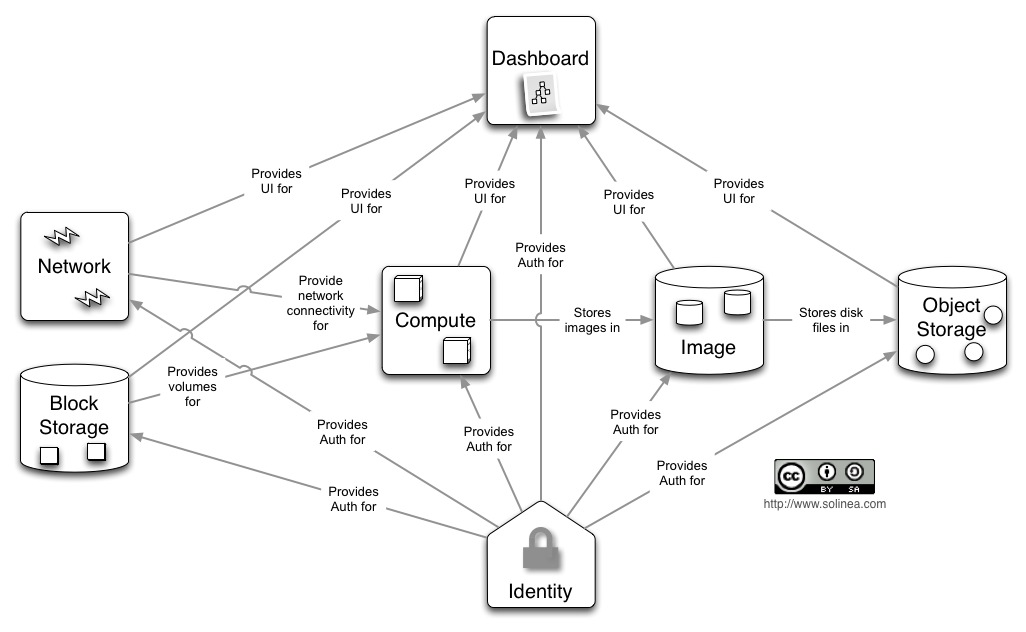
\includegraphics[width=\textwidth]{architecture-simple.jpg}
    \end{center}
  \end{frame}

  \begin{frame}
    \frametitle{Interface web / Dashboard : Horizon}
    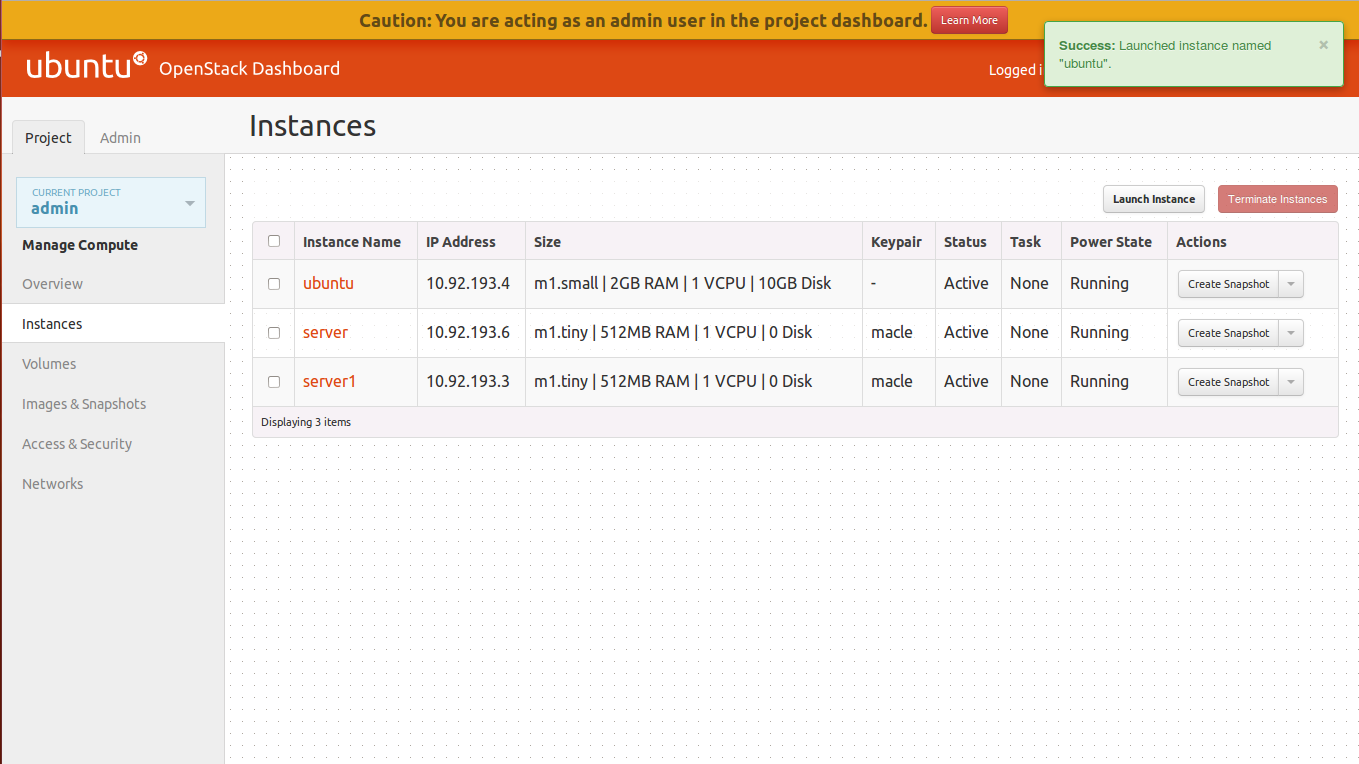
\includegraphics[width=\textwidth]{horizon.png}
  \end{frame}

  \begin{frame}
    \frametitle{Ressources}
    \begin{itemize}
      \item \url{http://docs.openstack.org/}
      \item \url{https://ask.openstack.org}
      \item openstack@lists.openstack.org
      \item \#openstack@Freenode
      \item \url{http://api.openstack.org/}
      \item Communauté française :
      \begin{itemize}
        \item \url{http//openstack.fr/}
        \item openstack-fr@lists.openstack.org
        \item \#openstack-fr@Freenode
		\item Association
      \end{itemize}
    \end{itemize}
  \end{frame}

  \subsection[DevStack]{DevStack : faire tourner rapidement un OpenStack}

  \begin{frame}
    \frametitle{Utilité de DevStack}
    \begin{itemize}
      \item Déployer rapidement un OpenStack
      \item Utilisé par les développeurs pour tester leurs changements
      \item Utilisé pour faire des démonstrations
      \item Utilisé pour tester les APIs sans se préoccuper du déploiement
      \item Ne doit PAS être utilisé pour de la production
    \end{itemize}
  \end{frame}

  \begin{frame}
    \frametitle{Fonctionnement de DevStack}
    \begin{itemize}
      \item Un script shell qui fait tout le travail : stack.sh
      \item Un fichier de configuration : local.conf
      \item Installe toute les dépendances nécessaires (paquets)
      \item Clone les dépôts git (branche master par défaut)
      \item Lance tous les composants dans un screen
    \end{itemize}
  \end{frame}

  \begin{frame}[containsverbatim]
    \frametitle{Configuration : local.conf}
    Exemple
\begin{verbatim}
[[local|localrc]]
ADMIN_PASSWORD=secrete
DATABASE_PASSWORD=$ADMIN_PASSWORD
RABBIT_PASSWORD=$ADMIN_PASSWORD
SERVICE_PASSWORD=$ADMIN_PASSWORD
SERVICE_TOKEN=a682f596-76f3-11e3-b3b2-e716f9080d50
#FIXED_RANGE=172.31.1.0/24
#FLOATING_RANGE=192.168.20.0/25
#HOST_IP=10.3.4.5
\end{verbatim}
  \end{frame}

  \begin{frame}
    \frametitle{Conseils d'utilisation}
    \begin{itemize}
      \item DevStack installe beaucoup de choses sur la machine
      \item Il est recommandé de travailler dans une VM
      \item Pour tester tous les composants OpenStack dans de bonnes conditions, plusieurs Go de RAM sont nécessaires
      \item L'utilisation de Vagrant est conseillée
    \end{itemize}
  \end{frame}

  \subsection[Utilisation]{Utiliser OpenStack}

  \begin{frame}
    \frametitle{Le principe}
    \begin{itemize}
      \item Toutes les fonctionnalités sont accessibles par l'API
      \item Les clients (y compris Horizon) utilisent l'API
      \item Des crédentials sont nécessaires
      \begin{itemize}
        \item API OpenStack : utilisateur + mot de passe + tenant
      \end{itemize}
    \end{itemize}
  \end{frame}

  \begin{frame}
    \frametitle{Accès aux APIs}
    \begin{itemize}
      \item Direct, en HTTP, via des outils comme curl
      \item Avec une bibliothèque
      \begin{itemize}
        \item Les implémentations officielles en Python
        \item D'autres implémentations pour d'autres langages (exemple : jclouds)
      \end{itemize}
      \item Avec les outils officiels en ligne de commande
      \item Avec Horizon
    \end{itemize}
  \end{frame}

  \begin{frame}
    \frametitle{Clients officiels}
    \begin{itemize}
      \item Le projet fournit des clients officiels : python-PROJETclient
      \item Bibliothèques Python
      \item Outils CLI
      \begin{itemize}
        \item L'authentification se fait en passant les credentials par paramètres ou variables d'environnement
        \item L'option --debug affiche la communication HTTP
      \end{itemize}
    \end{itemize}
  \end{frame}

  \section{Déployer OpenStack}

  \begin{frame}
    \frametitle{Ce qu'on va voir}
    \begin{itemize}
      \item Installer OpenStack à la main \url{http://docs.openstack.org/icehouse/install-guide/install/apt/content/}
      \item Donc comprendre son fonctionnement
      \item Tour d'horizon des solutions de déploiement
    \end{itemize}
  \end{frame}

  \begin{frame}
    \frametitle{Architecture détaillée}
    \begin{center}
      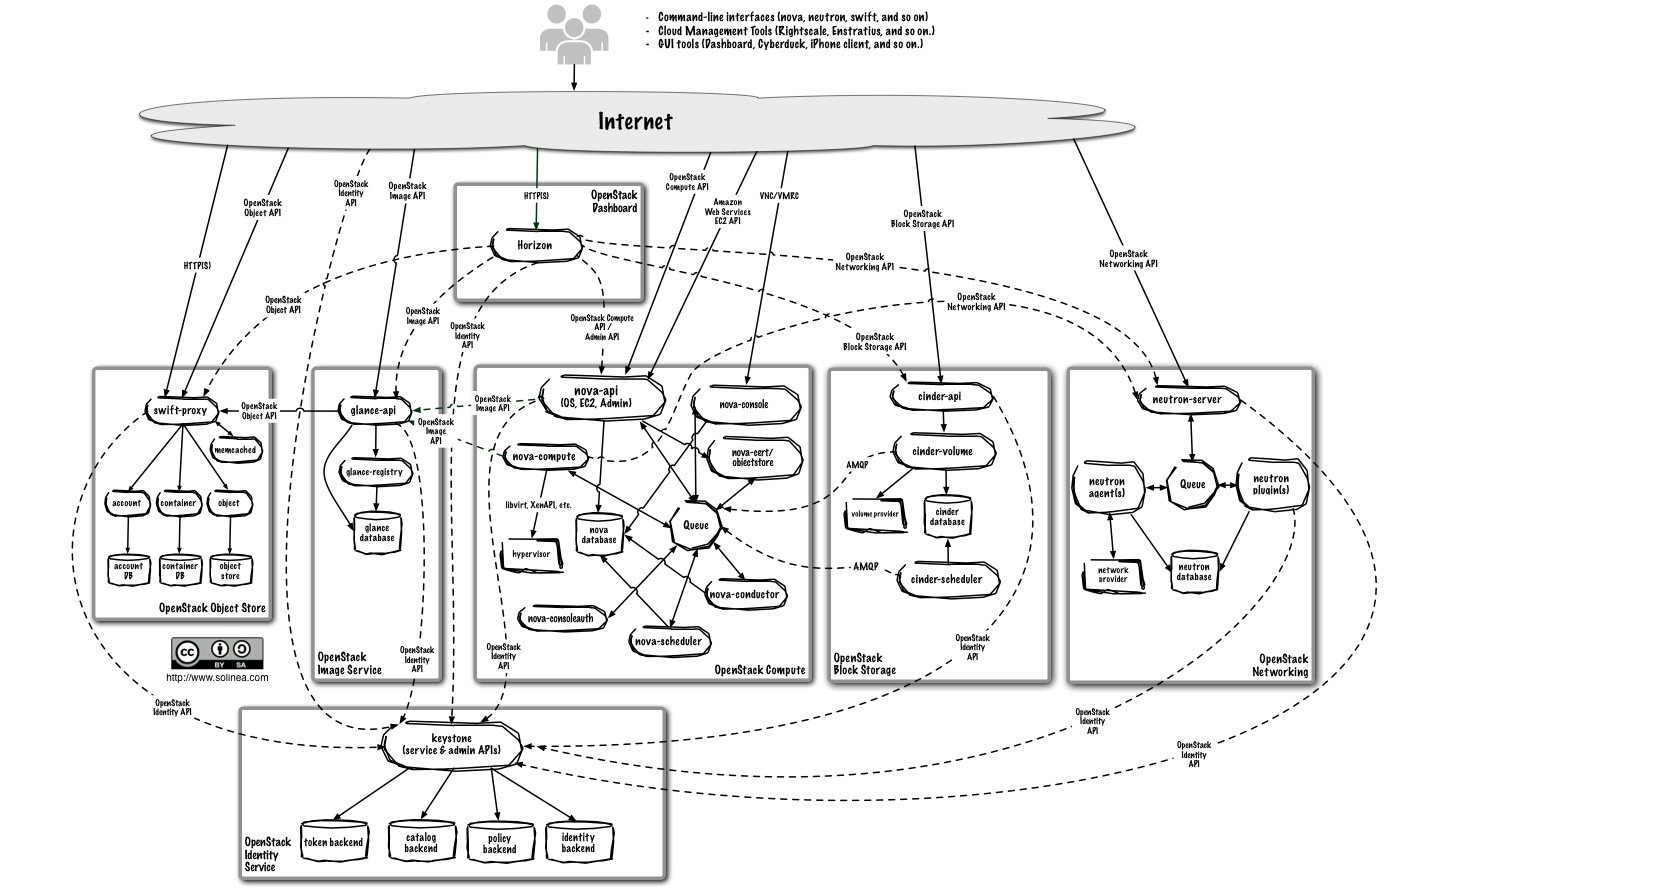
\includegraphics[width=\textwidth]{architecture.jpg}
    \end{center}
  \end{frame}

  \begin{frame}
    \frametitle{Quelques éléments de configuration généraux}
    \begin{itemize}
      \item Tous les composants doivent être configurés pour communiquer avec Keystone
      \item La plupart doivent être configurés pour communiquer avec MySQL et RabbitMQ
      \item Les composants découpés en plusieurs services ont souvent un fichier de configuration par service
      \item api-paste.ini contient des paramètres concernant le service API
    \end{itemize}
  \end{frame}

  \subsection[Les briques nécessaires]{Les briques nécessaires}
  \begin{frame}
    \frametitle{Système d'exploitation}
    \begin{itemize}
      \item OS Linux avec Python
      \item Historiquement : Ubuntu
      \item Red Hat s'est largement rattrapé
      \item SUSE, etc.
    \end{itemize}
  \end{frame}

  \begin{frame}
    \frametitle{Python}
    \begin{center}
      
\includegraphics{python-powered.png}
    \end{center}
    \begin{itemize}
      \item OpenStack est aujourd'hui compatible Python 2.7
      \item Afin de ne pas réinventer la roue, beaucoup de dépendances sont nécessaires
      \item Un travail de portage vers Python 3 est en cours
    \end{itemize}
  \end{frame}

  \begin{frame}
    \frametitle{Base de données}
    \begin{itemize}
      \item Permet de stocker la majorité des données gérées par OpenStack
      \item Chaque composant a sa propre base
      \item OpenStack utilise l'ORM Python SQLAlchemy
      \item Support théorique équivalent à celui de SQLAlchemy
      \item MySQL est l'implémentation la plus largement testée et utilisée
      \item SQLite est principalement utilisé dans le cadre de tests et démo
      \item Certains déploiements fonctionnent avec PostgreSQL
    \end{itemize}
  \end{frame}

  \begin{frame}
    \frametitle{Pourquoi l'utilisation de SQLAlchemy}
    \begin{center}
      
\includegraphics[width=10cm]{sqlalchemy-logo.png}
    \end{center}
    \begin{itemize}
      \item Support de multiples BDD
      \item Gestion des migrations
    \end{itemize}
    \begin{center}
      
\includegraphics{mysql-logo.png}
    \end{center}
  \end{frame}

  \begin{frame}
    \frametitle{Passage de messages}
    \begin{itemize}
      \item AMQP : Advanced Message Queuing Protocol
      \item Messages, file d'attente, routage
      \item Les processus OpenStack communiquent via AMQP
      \item Plusieurs implémentations possibles : Qpid, 0MQ, etc.
      \item RabbitMQ par défaut
    \end{itemize}
  \end{frame}

  \begin{frame}
  \frametitle{RabbitMQ}
    \begin{center}
      
\includegraphics{rabbitmq-logo.png}
    \end{center}
    \begin{itemize}
      \item RabbitMQ est implémenté en Erlang
      \item Une machine virtuelle Erlang est donc nécessaire
    \end{itemize}
  \end{frame}

  \begin{frame}
    \frametitle{"Hello world" RabbitMQ}
    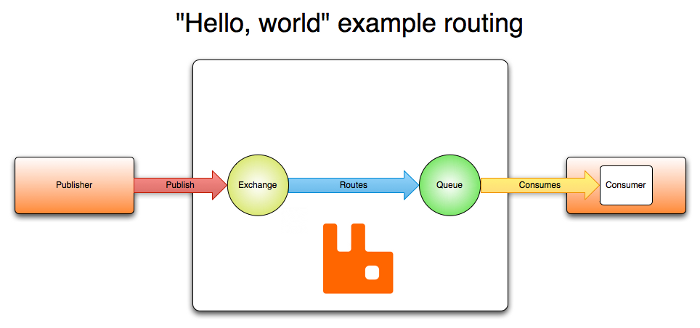
\includegraphics[width=\textwidth]{rabbitmq-schema.png}
  \end{frame}

  \subsection[Keystone]{Keystone : Authentification, autorisation et catalogue de services}

  \begin{frame}
    \frametitle{Principes}
    \begin{itemize}
      \item Annuaire des utilisateurs et des groupes
      \item Catalogue de services
      \item Gère l'authentification et l'autorisation
      \item Support des domaines dans l'API v3
      \item Fournit un token à l'utilisateur
    \end{itemize}
  \end{frame}

  \begin{frame}
    \frametitle{API}
    \begin{itemize}
      \item API admin : port 35357
      \item API utilisateur : port 5000
      \item Deux versions : v2 (actuelle) et v3 (future)
      \item Gère \textit{utilisateurs}, \textit{groupes}, \textit{domaines} (APIv3)
      \item Les utilisateurs ont des \textit{rôles} sur des \textit{tenants} (projets)
    \end{itemize}
  \end{frame}

  \begin{frame}
    \frametitle{Scénario d'utilisation typique}
    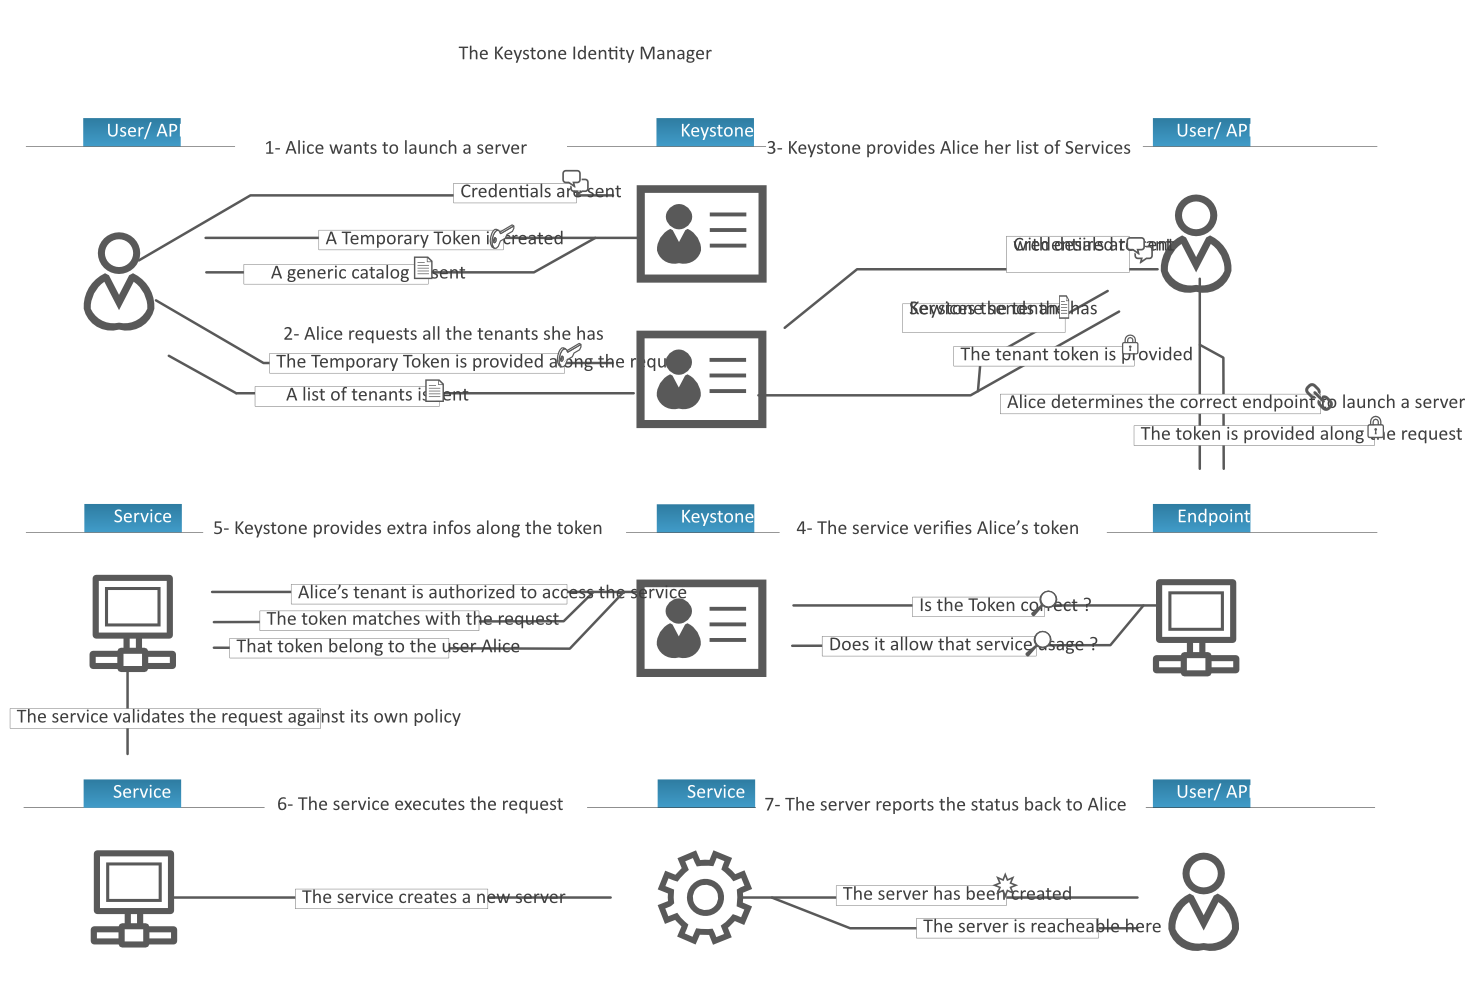
\includegraphics[width=\linewidth]{keystone-scenario.png}
  \end{frame}

  \begin{frame}
    \frametitle{Installation et configuration}
    \begin{itemize}
      \item Paquet : keystone
      \item Configuration d'un token ADMIN pour la configuration initiale
      \item Backends : choix de SQL ou LDAP (ou AD)
      \item Configurer les différents services
      \item Policy.json
      \item Services et endpoints
      \item Utilisateurs, groupes, domaines
    \end{itemize}
  \end{frame}

  \begin{frame}[containsverbatim]
    \frametitle{Enregistrer un service et son endpoint}
    Il faut renseigner l'existence des différents services (catalogue) dans Keystone :
    \begin{verbatim}
$ keystone service-create --name=cinderv2 --type=volumev2 \
  --description="Cinder Volume Service V2"
$ keystone endpoint-create \
  --region=myRegion
  --service-id=...
  --publicurl=http://controller:8776/v2/%\(tenant_id\)s \
  --internalurl=http://controller:8776/v2/%\(tenant_id\)s \
  --adminurl=http://controller:8776/v2/%\(tenant_id\)s
    \end{verbatim}
  \end{frame}

  \begin{frame}[containsverbatim]
    \frametitle{Tester}
\begin{verbatim}
$ keystone service-list
...
$ keystone user-list
...
$ keystone token-get
...
\end{verbatim}
  \end{frame}

  \subsection[Nova]{Nova : Compute}

  \begin{frame}
    \frametitle{Principes}
    \begin{itemize}
      \item Gère les instances
      \item IP flottantes, groupes de sécurité
      \item Les instances sont créées à partir des images fournies par Glance
      \item Les interfaces réseaux des instances sont associées à des ports Neutron
    \end{itemize}
  \end{frame}

  \begin{frame}
    \frametitle{Interactions avec les autres composants}
    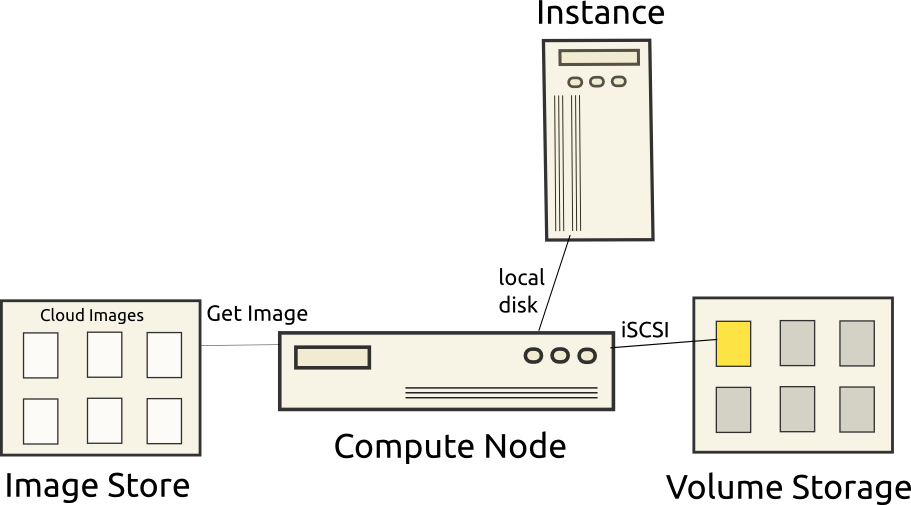
\includegraphics[width=\textwidth]{compute-node.png}
  \end{frame}

  \begin{frame}
    \frametitle{API}
    Gère :
    \begin{itemize}
      \item Instances
      \item Flavors
      \item Security Groups
      \item Floating IPs
    \end{itemize}
    Les instances sont redimensionnables et migrables.
  \end{frame}

  \begin{frame}
    \frametitle{Rôle des flavors}
    \begin{itemize}
      \item Équivalent des "instance types" d'AWS
      \item Définit un modèle d'instance en termes de CPU, RAM, disque
    \end{itemize}
  \end{frame}

  \begin{frame}
    \frametitle{Nova api}
    \begin{itemize}
      \item Double rôle
      \item API de manipulation des instances par l'utilisateur
      \item API à destination des instances : API de metadata
      \item L'API de metadata doit être accessible à l'adresse http://169.254.169.254/
      \item L'API de metadata fournit des informations de configuration personnalisées à chacune des instances
    \end{itemize}
  \end{frame}

  \begin{frame}
    \frametitle{Nova compute}
    \begin{itemize}
      \item Exécute les machines virtuelles
      \item Tire partie de libvirt ou d'autres APIs comme XenAPI
      \item Drivers : libvirt, XenAPI, VMWare ESX, Docker
      \item Permet de récupérer les logs de la console et une console VNC
    \end{itemize}
  \end{frame}

  \begin{frame}
    \frametitle{Nova scheduler}
    \begin{itemize}
      \item Service qui distribue les demandes d'instances sur les noeuds compute
      \item Filter, Chance, Multi Scheduler
      \item Filtres, par défaut : AvailabilityZoneFilter,RamFilter,ComputeFilter
      \item Tri par poids, par défaut : RawWeigher
    \end{itemize}
  \end{frame}

  \begin{frame}
    \frametitle{Le scheduler Nova en action}
    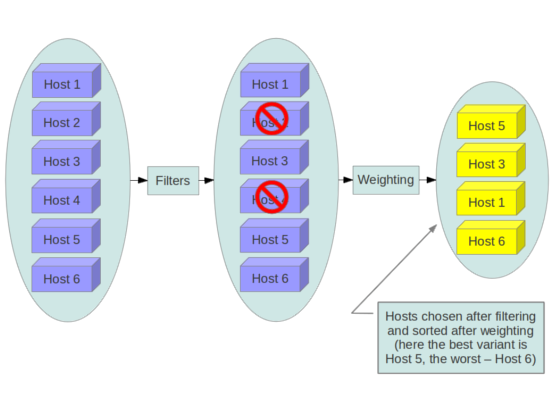
\includegraphics[width=\textwidth]{scheduling-schema.png}
  \end{frame}

  \begin{frame}
    \frametitle{Nova conductor}
    \begin{itemize}
      \item Service facultatif qui améliore la sécurité
      \item Fait office de proxy entre les noeuds compute et la BDD
      \item Les noeuds compute, vulnérables, n'ont donc plus d'accès à la BDD
    \end{itemize}
  \end{frame}

  \begin{frame}[containsverbatim]
    \frametitle{Tester}
\begin{verbatim}
$ nova list
...
$ nova create
...
\end{verbatim}
  \end{frame}

  \subsection[Glance]{Glance : Registre d'images}

  \begin{frame}
    \frametitle{Principes}
    \begin{itemize}
      \item Registre d'images (et des snapshots)
      \item Propriétés sur les images
      \item Est utilisé par Nova pour démarrer des instances
      \item Peut utiliser Swift comme back-end de stockage
    \end{itemize}
  \end{frame}

  \begin{frame}
    \frametitle{Propriétés des images dans Glance}
    L'utilisateur peut définir un certain nombre de propriétés dont certaines seront utilisées lors de l'instanciation
    \begin{itemize}
      \item Type d'image
      \item Architecture
      \item Distribution
      \item Version de la distribution
      \item Espace disque minimum
      \item RAM minimum
      \item Publique ou non
    \end{itemize}
  \end{frame}

  \begin{frame}
    \frametitle{Types d'images}
    Glance supporte un large éventail de types d'images, limité par le support de l'hyperviseur sous-jacent à Nova
    \begin{itemize}
      \item raw
      \item qcow2
      \item ami
      \item vmdk
      \item iso
    \end{itemize}
  \end{frame}

  \begin{frame}
    \frametitle{Backends}
    \begin{itemize}
      \item Swift ou S3
      \item Ceph
      \item HTTP
      \item Répertoire local
    \end{itemize}
  \end{frame}

  \begin{frame}
    \frametitle{Installation}
    \begin{itemize}
      \item Paquet glance-api : fournit l'API
      \item Paquet glance-registry : démon du registre d'images en tant que tel
    \end{itemize}
  \end{frame}

  \begin{frame}[containsverbatim]
    \frametitle{Tester}
\begin{verbatim}
$ glance image-list
...
$ glance image-create
...
\end{verbatim}
  \end{frame}

  \subsection[Neutron]{Neutron : Réseau en tant que service}

  \begin{frame}
    \frametitle{Principes}
    \begin{itemize}
      \item SDN
      \item Auparavant Quantum et nova-network
      \item neutron-server : fournit l'API
      \item Agent DHCP : fournit le service de DHCP pour les instances
      \item Agent L3 : gère la couche 3 du réseau, le routage
      \item Plugin : OpenVSwitch par défaut, d'autres implémentations libres/propriétaires, logicielles/matérielles existent
    \end{itemize}
  \end{frame}

  \begin{frame}
    \frametitle{Fonctionnalités supplémentaires}
    Outre les fonctions réseau de base niveaux 2 et 3, Neutron peut fournir d'autres services :
    \begin{itemize}
      \item Load Balancing (HAProxy, ...)
      \item Firewall (vArmour, ...)
      \item VPN (Openswan, ...)
    \end{itemize}
    Ces fonctionnalités se basent également sur des plugins
  \end{frame}

  \begin{frame}
    \frametitle{API}
    L'API permet notamment de manipuler ces ressources
    \begin{itemize}
      \item Réseau : niveau 2
      \item Subnet : niveau 3
      \item Port
    \end{itemize}
    Les ports peuvent correspondre à des interfaces d'instance
  \end{frame}

  \begin{frame}
    \frametitle{Plugins ML2}
    \begin{itemize}
      \item Modular Layer 2
      \item OpenVSwitch
      \item OpenDaylight
      \item Contrail, OpenContrail
      \item Nuage Networks
      \item cf. OpenFlow
    \end{itemize}
  \end{frame}

  \begin{frame}
    \frametitle{Implémentation}
    \begin{itemize}
      \item Neutron tire partie des namespaces réseaux du noyau Linux pour permettre l'IP overlapping
      \item Le proxy de metadata est un composant qui permet aux instances isolées dans leur réseau de joindre l'API de metadata fournie par Nova
    \end{itemize}
  \end{frame}

  \begin{frame}
    \frametitle{Schéma}
    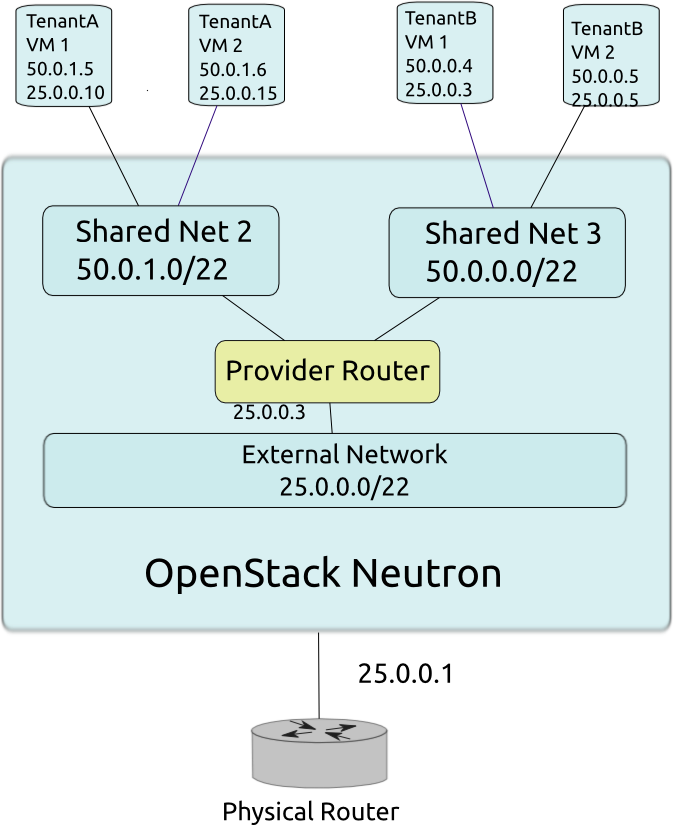
\includegraphics[width=\textwidth,height=\textheight]{neutron-schema.png}
  \end{frame}

  \subsection[Cinder]{Cinder : Stockage block}

  \begin{frame}
    \frametitle{Principes}
    \begin{itemize}
      \item Auparavant nova-volume
      \item Fournit des volumes (stockage block) attachables aux instances
      \item Gère différents types de volume
      \item Gère snapshots et backups de volumes
      \item Attachement via iSCSI par défaut
    \end{itemize}
  \end{frame}

  \begin{frame}
    \frametitle{Du stockage partagé ?}
    \begin{itemize}
      \item Cinder n'est \textbf{pas} une solution de stockage partagé comme NFS
      \item OpenStack (tout comme AWS) ne fournit pas de solution \textit{NFS as a Service}
      \item Cf. le projet Manila
    \end{itemize}
  \end{frame}

  \begin{frame}
    \frametitle{Utilisation}
    \begin{itemize}
      \item Volume supplémentaire (et stockage persistant) sur une instance
      \item Boot from volume : l'OS est sur le volume
      \item Fonctionnalité de backup vers un object store (Swift ou Ceph)
    \end{itemize}
  \end{frame}

  \begin{frame}
    \frametitle{Installation}
    \begin{itemize}
      \item Paquet cinder-api : fournit l'API
      \item Paquet cinder-volume : création et gestion des volumes
      \item Paquet cinder-scheduler : distribue les demandes de création de volume
      \item Paquet cinder-backup : backup vers un object store
    \end{itemize}
  \end{frame}

  \begin{frame}
    \frametitle{Backends}
    \begin{itemize}
      \item Utilisation de plusieurs backends en parallèle possible
      \item LVM (par défaut)
      \item GlusterFS
      \item Ceph
      \item Systèmes de stockage propriétaires type NetApp
    \end{itemize}
  \end{frame}

  \subsection[Horizon]{Horizon : Dashboard web}

  \begin{frame}
    \frametitle{Principes}
    \begin{itemize}
      \item Utilise les APIs existantes pour fournir une interface
      \item Horizon est un module Django
      \item OpenStack Dashboard est l'implémentation officielle de ce module
    \end{itemize}
    \begin{center}
      
\includegraphics[width=8cm]{django-logo.png}
    \end{center}
  \end{frame}

  \begin{frame}
    \frametitle{Configuration}
    \begin{itemize}
      \item local\_settings.py
      \item Les services apparaissent dans Horizon s'ils sont répertoriés dans le catalogue de services de Keystone
    \end{itemize}
  \end{frame}

  \begin{frame}
    \frametitle{Utilisation}
    \begin{itemize}
      \item Une zone "admin" restreinte
      \item Une interface par tenant
    \end{itemize}
  \end{frame}

  \subsection[Swift]{Swift : Stockage objet}

  \begin{frame}
    \frametitle{Principes}
    \begin{itemize}
      \item SDS : Software Defined Storage
      \item Utilisation de commodity hardware
      \item Théorème CAP : on en choisit deux
      \item Accès par les APIs
      \item Architecture totalement acentrée
      \item Pas de base de données centrale
    \end{itemize}
  \end{frame}

  \begin{frame}
    \frametitle{Implémentation}
    \begin{itemize}
      \item Proxy : serveur API par lequel passent toutes les requêtes
      \item Object server : serveur de stockage
      \item Container server : maintient des listes d'objects dans des containers
      \item Account server : maintient des listes de containers dans des accounts
      \item Chaque objet est répliqué n fois (3 par défaut)
    \end{itemize}
  \end{frame}

  \begin{frame}
    \frametitle{Le ring}
    \begin{itemize}
      \item Problème : comment décider quelle donnée va sur quel object server
      \item Le ring est découpé en partitions
      \item On situe chaque donnée dans le ring afin de déterminer sa partition
      \item Une partition est associée à plusieurs serveurs
    \end{itemize}
  \end{frame}

  \begin{frame}
    \frametitle{Schéma}
    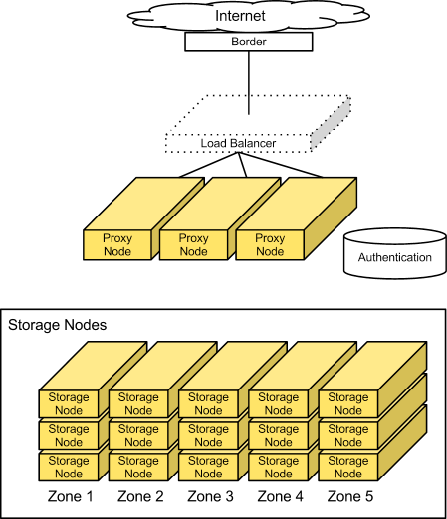
\includegraphics[width=\textwidth,height=\textheight]{swift-schema.png}
  \end{frame}

  \subsection[Ceilometer]{Ceilometer : Collecte de métriques}

  \begin{frame}
    \frametitle{Surveiller l'utilisation de son infrastructure avec Ceilometer}
    \begin{itemize}
      \item Indexe différentes métriques concernant l'utilisation des différents services du cloud
      \item Fournit des APIs permettant de récupérer ces données
      \item Base pour construire des outils de facturation
      \item Utilise MongoDB (par défaut) pour le stockage
    \end{itemize}
  \end{frame}

  \subsection[Heat]{Heat : Orchestration des ressources}

  \begin{frame}
    \frametitle{Orchestrer son infrastructure avec Heat}
    \begin{itemize}
      \item Équivalent d'Amazon Cloud Formation
      \item Orchestrer les ressources compute, storage, network, etc.
      \item Doit se coupler avec cloud-init\pause
      \item Description de son infrastructure dans un fichier template, format JSON (CFN) ou YAML (HOT)
    \end{itemize}
  \end{frame}

  \begin{frame}
    \frametitle{Autoscaling avec Heat}
    Heat implémente la fonctionnalité d'autoscaling
    \begin{itemize}
      \item Se déclenche en fonction des alarmes produites par Ceilometer
      \item Entraine la création de nouvelles instances
    \end{itemize}
  \end{frame}

  \begin{frame}[containsverbatim]
    \frametitle{Un template HOT}
\begin{verbatim}
heat_template_version: 2013-05-23

description: Simple template to deploy a single compute instance

resources:
  my_instance:
    type: OS::Nova::Server
    properties:
      key_name: my_key
      image: F18-x86_64-cfntools
      flavor: m1.small
\end{verbatim}
  \end{frame}

  \subsection[Trove]{Trove : Database as a Service}

  \begin{frame}
    \frametitle{Principe}
    \begin{itemize}
      \item Fournit des bases de données relationnelles, à la AWS RDS
      \item A vocation à supporter des bases NoSQL aussi
      \item Gère notamment MySQL comme back-end
      \item Se repose sur Nova pour les instances dans lesquelles se fait l'installation d'une BDD
    \end{itemize}
  \end{frame}

  \begin{frame}
    \frametitle{Services}
    \begin{itemize}
      \item trove-api : API
      \item trove-taskmanager : gère les instances BDD
      \item trove-guestagent : agent interne à l'instance
    \end{itemize}
  \end{frame}

  \subsection[Designate]{Designate : DNS as a Service}

  \begin{frame}
    \frametitle{Principe}
    \begin{itemize}
      \item Équivalent d'AWS Route 53
      \item Gère différents backends : BIND, etc.
    \end{itemize}
  \end{frame}

  \subsection[Les autres]{Quelques autres composants intéressants}

  \begin{frame}
    \frametitle{Ironic}
    \begin{itemize}
      \item Anciennement Nova bare-metal
      \item Permet le déploiement d'instance sur des machines physiques (plutôt que VMs)
      \item Repose sur des technologies telles que PXE, TFTP
    \end{itemize}
  \end{frame}

  \begin{frame}
    \frametitle{Oslo, ou OpenStack common}
    \begin{itemize}
      \item Oslo contient le code commun à plusieurs composants d'OpenStack
      \item Son utilisation est transparente pour le déployeur
    \end{itemize}
  \end{frame}

  \begin{frame}
    \frametitle{rootwrap}
    \begin{itemize}
      \item Wrapper pour l'utilisation de commandes en root
      \item Configuration au niveau de chaque composant qui l'utilise
      \item Permet d'écrire des filtres sur les commandes
    \end{itemize}
  \end{frame}

  \begin{frame}
    \frametitle{TripleO}
    \begin{itemize}
      \item OpenStack On OpenStack
      \item Objectif : pouvoir déployer un cloud OpenStack (overcloud) à partir d'un cloud OpenStack (undercloud)
      \item Autoscaling du cloud lui-même : déploiement de nouveaux noeuds compute lorsque cela est nécessaire
      \item Fonctionne conjointement avec Ironic pour le déploiement bare-metal
    \end{itemize}
  \end{frame}

  \begin{frame}
    \frametitle{Tempest}
    \begin{itemize}
      \item Suite de tests d'un cloud OpenStack
      \item Effectue des appels à l'API et vérifie le résultat
      \item Est très utilisé par les développeurs via l'intégration continue
      \item Le déployeur peut utiliser Tempest pour vérifier la bonne conformité de son cloud
    \end{itemize}
  \end{frame}

  \subsection[Déployer en production]{Bonnes pratiques pour un déploiement en production}

  \begin{frame}
    \frametitle{Quels composants dois-je installer ?}
      \begin{itemize}
        \item Keystone est indispensable
        \item L'utilisation de Nova va de paire avec Glance et Neutron
        \item Cinder s'avérera souvent utile
        \item Ceilometer et Heat vont souvent ensemble
        \item Swift est indépendant des autres composants
      \end{itemize}
  \end{frame}

  \begin{frame}
    \frametitle{Penser dès le début aux choix structurants}
    \begin{itemize}
      \item Distribution et méthode de déploiement
      \item Hyperviseur
      \item Réseau : quelle architecture et quels drivers
      \item Politique de mise à jour
    \end{itemize}
  \end{frame}

  \begin{frame}
    \frametitle{Les différentes méthodes d'installation}
    \begin{itemize}
      \item DevStack est à oublier pour la production
      \item TripleO est encore trop jeune
      \item Le déploiement à la main comme vu précédemment n'est pas recommandé car peu maintenable
      \item Distributions OpenStack packagées et prêtes à l'emploi
      \item Distributions classiques et gestion de configuration
    \end{itemize}
  \end{frame}

  \begin{frame}
    \frametitle{Assigner des rôles aux machines}
    Beaucoup de documentations font référence à ces rôles :
    \begin{itemize}
      \item Controller node : APIs, BDD, AMQP
      \item Network node : Routeur
      \item Compute node : Hyperviseur
    \end{itemize}
    Ce modèle simplifié n'est pas HA.
  \end{frame}

  \begin{frame}
    \frametitle{Haute disponbilité}
    Haut disponibilité de l'IaaS
    \begin{itemize}
      \item MySQL, RabbitMQ : HA classique (Galera, Clustering)
      \item Les services APIs sont stateless et HTTP : scale out et load balancers
      \item La plupart des autres services OpenStack sont capables de scale out également
    \end{itemize}
    Guide HA : \url{http://docs.openstack.org/high-availability-guide/content/}
  \end{frame}

  \begin{frame}
    \frametitle{Considérations pour une environnement de production}
    \begin{itemize}
      \item Des URLs uniformes pour toutes les APIs : utiliser un reverse proxy
      \item Utilisation des quotas
      \item Prévoir les bonnes volumétries, notamment pour les données Ceilometer
      \item Monitoring
    \end{itemize}
    Guide Operations : \url{http://docs.openstack.org/trunk/openstack-ops/content/}
  \end{frame}

  \begin{frame}
  \frametitle{Découpage réseau}
    \begin{itemize}
      \item Management network : réseau d'administration
      \item Data network : réseau pour la communication inter instances
      \item External network : réseau externe, dans l'infrastructure réseau existante
      \item API network : réseau contenant les endpoints API
    \end{itemize}
  \end{frame}

  \begin{frame}
    \frametitle{Considérations liées à la sécurité}
    \begin{itemize}
      \item Indispensable : HTTPS sur l'accès des APIs à l'extérieur
      \item Sécurisation des communications MySQL et RabbitMQ
      \item Un accès MySQL par base et par service
      \item Un utilisateur Keystone par service
      \item Limiter l'accès en lecture des fichiers de configuration (mots de passe, token)
    \end{itemize}
  \end{frame}

  \begin{frame}
    \frametitle{Segmenter son cloud}
    \begin{itemize}
      \item Host aggregates : machines physiques avec des caractéristiques similaires
      \item Availability zones : machines dépendantes d'une même source électrique, d'un même switch, d'un même DC, etc.
      \item Regions : chaque région a son API
      \item Cells : permet de regrouper plusieurs cloud différents sous une même API
    \end{itemize}
  \end{frame}

  \begin{frame}
    \frametitle{Host aggregates / agrégats d'hôtes}
    \begin{itemize}
      \item L'administrateur définit des agrégats via l'API
      \item 1 agrégat $\equiv$ 1 point commun, ex : GPU
      \item L'utilisateur peut choisir un agrégat à la création d'instance
    \end{itemize}
  \end{frame}

  \begin{frame}
    \frametitle{Availability zones / zones de disponibilité}
    \begin{itemize}
      \item Groupe d'hôtes
      \item Découpage en termes de disponibilité : Rack, Datacenter, etc.
      \item L'utiliser peut choisir une zone de disponibilité
      \item L'utilisateur peut demander à ce que des instances soient démarrer dans une même zone, ou au contraire dans des zones différentes
    \end{itemize}
  \end{frame}

  \begin{frame}
    \frametitle{Régions}
    \begin{itemize}
      \item Équivalent des régions d'AWS
      \item Un service peut avoir différents endpoints dans différentes régions
      \item Chaque région est autonome
      \item Cas d'usage : cloud de grande ampleur (comme certains clouds publics)
    \end{itemize}
  \end{frame}

  \begin{frame}
    \frametitle{Cellules / Cells}
    \begin{itemize}
      \item Fonctionnalité de Nova uniquement
      \item Un seul nova-api devant plusieurs cellules
      \item Chaque cellule a sa propre BDD et file de messages
      \item Ajoute un niveau de scheduling (choix de la cellule)
    \end{itemize}
  \end{frame}

  \begin{frame}
    \frametitle{Packaging d'OpenStack - Ubuntu}
    \begin{itemize}
      \item Le packaging est fait dans de multiples distributions, RPM, DEB et autres\pause
      \item Ubuntu est historiquement la plateforme de référence pour le développement d'OpenStack
      \item Le packaging dans Ubuntu suit de près le développement d'OpenStack, et des tests automatisés sont réalisés
      \item Canonical fournit la Ubuntu Cloud Archive, qui met à disposition la dernière version d'OpenStack pour la dernière Ubuntu LTS
    \end{itemize}
  \end{frame}

  \begin{frame}
    \frametitle{Ubuntu Cloud Archive}
    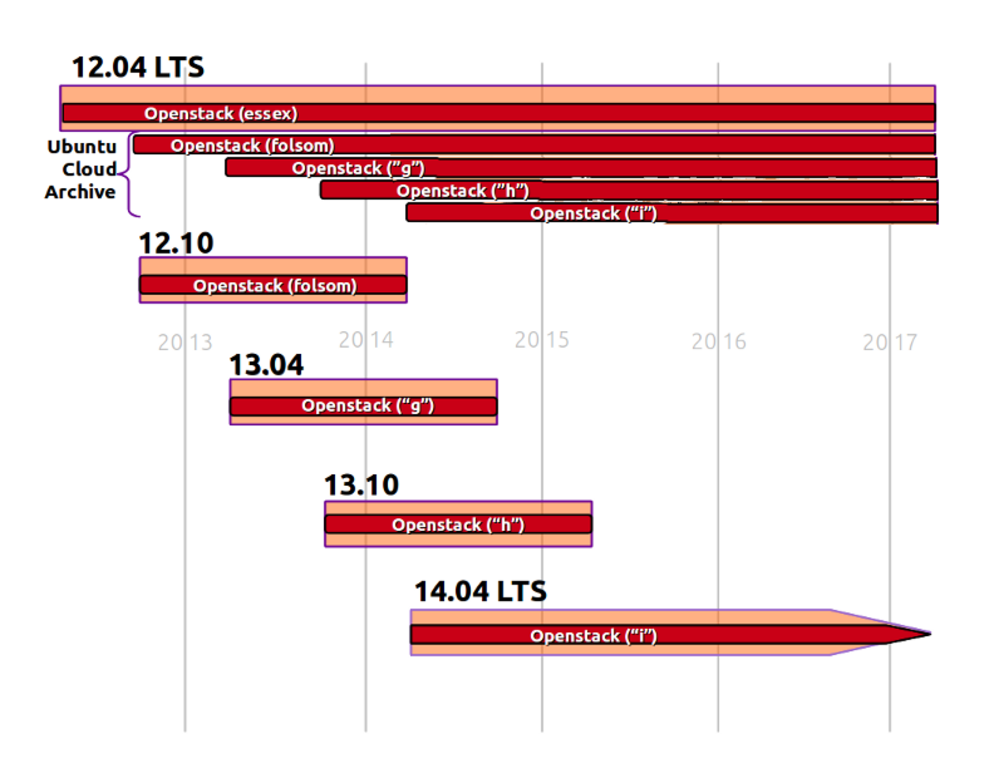
\includegraphics{ubuntu-cloud-archive.png}
  \end{frame}

  \begin{frame}
    \frametitle{Packaging d'OpenStack dans les autres distributions}
    \begin{itemize}
      \item OpenStack est intégré dans les dépôts officiels de Debian
      \item Red Hat propose RHOS
      \item Comme Ubuntu, le cycle de release de Fedora est synchronisé avec celui d'OpenStack
    \end{itemize}
  \end{frame}

  \begin{frame}
    \frametitle{Les distributions OpenStack}
    \begin{itemize}
      \item StackOps
      \item Mirantis
      \item HP
      \item etc.
    \end{itemize}
  \end{frame}

  \begin{frame}
    \frametitle{Déploiement bare metal}
    \begin{itemize}
      \item Le déploiement des hôtes physiques OpenStack peut se faire à l'aide d'outils dédiés\pause
      \item Canonical/Ubuntu propose MaaS : Metal as a Service
      \item Dell propose Crowbar
      \item eDeploy (eNovance)
    \end{itemize}
  \end{frame}

  \begin{frame}
    \frametitle{Gestion de configuration}
    \begin{itemize}
      \item Puppet, Chef, CFEngine, Saltstack, Ansible, etc.\pause
      \item Ces outils peuvent aider à déployer le cloud OpenStack
      \item ... mais aussi à gérer les instances (section suivante)
    \end{itemize}
  \end{frame}

  \begin{frame}
    \frametitle{Modules Puppet}
    \begin{itemize}
      \item PuppetLabs maintient (avec d'autres) des modules pour déployer OpenStack
      \item \url{https://forge.puppetlabs.com/puppetlabs/openstack}
    \end{itemize}
  \end{frame}

  \subsection[Problèmes]{Faire face aux problèmes}

  \begin{frame}
    \frametitle{Les réflexes en cas d'erreur ou de comportement erroné}
    \begin{itemize}
      \item Travaille-t-on sur le bon tenant ?
      \item Est-ce que l'API renvoie une erreur ? (le dashboard peut cacher certaines informations)
      \item Si nécessaire d'aller plus loin :
        \begin{itemize}
          \item Regarder les logs sur le cloud controller (/var/log/<composant/*.log)
          \item Regarder les logs sur le compute node et le network node si le problème est spécifique réseau/instance
          \item Éventuellement modifier la verbosité des logs dans la configuration
        \end{itemize}
    \end{itemize}
  \end{frame}

  \begin{frame}
    \frametitle{Est-ce un bug ?}
    \begin{itemize}
      \item Si le client CLI crash, c'est un bug\pause
      \item Si le dashboard web affiche une erreur 500, c'est peut-être un bug\pause
      \item Si les logs montrent une stacktrace Python, c'est un bug\pause
      \item Sinon, à vous d'en juger
    \end{itemize}
  \end{frame}

  \section{Tirer partie de l'IaaS}

  \begin{frame}
    \frametitle{Deux visions}
    Une fois un cloud IaaS en place, deux optiques possibles :
    \begin{itemize}
      \item Garder les mêmes pratiques tout en profitant du self service et de l'agilité de la solution
      \item Faire évoluer ses pratiquer, tant côté applicatif que système
    \end{itemize}
    "Pets vs Cattle"
  \end{frame}

  \subsection{Côté applications}

  \begin{frame}
    \frametitle{Adapter ou faire ses applications "cloud ready"}
    \begin{itemize}
      \item Stateless : permet de multiplier les routes d'accès à l'application
      \item Ne pas stocker les données en local, mais plutôt :
      \begin{itemize}
        \item Base de données
        \item Stockage objet
      \end{itemize}
    \item Utiliser des outils standards de journalisation
    \end{itemize}
  \end{frame}

  \subsection{Côté système}

  \begin{frame}
    \frametitle{Adopter une philosophie DevOps}
    \begin{itemize}
      \item Infrastructure as Code
      \item Scale out au lieu de scale up
      \item HA niveau application plutôt qu'infrastructure
    \end{itemize}
  \end{frame}

  \begin{frame}
    \frametitle{Utiliser des images cloud}
    Une image cloud c'est :
    \begin{itemize}
      \item Une image disque contenant un OS déjà installé
      \item Une image qui peut être instanciée en n machines sans erreur
      \item Un OS sachant parler à l'API de metadata du cloud (cloud-init)
    \end{itemize}
    La plupart des distributions fournissent aujourd'hui des images cloud.
  \end{frame}

  \begin{frame}
    \frametitle{Cloud-init}
    \begin{itemize}
      \item Cloud-init est un moyen de tirer partie de l'API de metadata, et notamment des user data
      \item L'outil est intégré par défaut dans la plupart des images cloud
      \item À partir des user data, cloud-init effectue les opérations de personnalisation de l'instance
      \item cloud-config est un format possible de user data
    \end{itemize}
  \end{frame}

  \begin{frame}[containsverbatim]
    \frametitle{Exemple cloud-config}
\begin{verbatim}
#cloud-config
mounts:
 - [ xvdc, /var/www ]
packages:
 - apache2
 - htop
\end{verbatim}
  \end{frame}

  \section*{Conclusion}
  \begin{frame}
    \frametitle{Conclusion}
    \begin{itemize}
      \item Le cloud révolutionne l'IT
      \item OpenStack est le projet libre phare sur la partie IaaS
      \item Déployer OpenStack n'est pas une mince affaire
      \item L'utilisation d'un cloud IaaS implique des changements de pratique
    \end{itemize}
  \end{frame}

\end{document}
